\chapter{Results}
\label{chap:results}
%Merk at vi egentlig mener at diskusjonen i seg selv er en del av resultatet! Bruk diskursjon som et underpunkt til resultat

\begin{comment}
\section{Results from the Spectrometer I} 
the wave spectrum from one of the types. This can be compared to the associated colors wave spectrum. 
\section{Results from the Spectrometer II}
Comparing the signature of two different types of plastic (de gjennomsiktige pelletsene), which more or less have the same signature
\section{Principal Component Analysis I}
Using the different types of plastic only

\section{Principal Component Analysis II} 
The plastic types compared with algae

\section{The Final Method} 
\end{comment}

\section{PCA - Introduce and discuss figures}
The results from the PCA of the measurements showed no clear clusters or trends that would make it possible to distinguish individual types of plastic at this stage. The plot below shows the principal component analysis done on the results from scanning the plastic samples using hyper spectral imaging. The horizontal axis of the plot shows the first principal component and the percentage of the variables it explains, while the vertical axis shows the second principal component and its percentage for explained variables. The rings around clusters with the same color, or samples of the same type, are the 95\% confidence interval of the type, i.e. 95\% of the samples should lie within the ring. These should therefore clearly indicate whether there are any clusters depicting patterns in the sample data. Finally, the colored arrows on the circle centered in (0, 0) depict the direction of the increasing level of that color. The following along the direction indicated by the red arrow shows an increasing level of the color red in the sample, while following the blue arrow shows an increasing level of the color blue etc.The tested variables were previously presented in the \textit{Method} section.

\subsection{PCA with all Plastic Samples}
Figure \ref{fig:PCA_plastics_full_doub_cont} shows the contributions from the different wave lengths to the two principal components. The horizontal axis represent the wave lengths and the vertical axis the contribution in percent. The dashed red line represent 0.253\% or the line that shows the exact equal contribution from all wavelengths. Integrating the line would result in $0.253\% \cdot (700 - 400)/(0.758) \approx 100\%$.%Dette er feil. det skal være 0.252 siden det er en måling hver 0.758 og ikke hver nanometer, så er det mer riktig på bildet.
Also, the color of the line depicts the color at that wavelength, the blue color of the line at 450 nm is the color of light with that specific wavelength. 
\\\\%Påpeke at selv der man ser clusters så er ikke dette fremtredende i den samme plasttypen, men heller på bakgrunn av den fargen plasten innehar. 
As can be seen in the plot in figure \ref{fig:PCA_plastics_only_full_scat}, PC1 accounts for over 90\% of the variance. From the signature and contribution of PC1 in figure \ref{fig:PCA_plastics_full_doub_cont} it is apparent that the 94.1\% descriptive property of the first principal component is not rooted in one wave length or in a combination of wave lengths. The even distribution over the spectrum visualize the fact that PC1 mainly describes the \textit{lightness} of the plastic. From the position of the different samples it is clear that the results are dominated by this fact. Due to the low variance of the second principal component, of only X \%, the vertical spread and thus the few clusters there are are not well described and may not be deemed representative.

\begin{figure}[H]
    \centering
    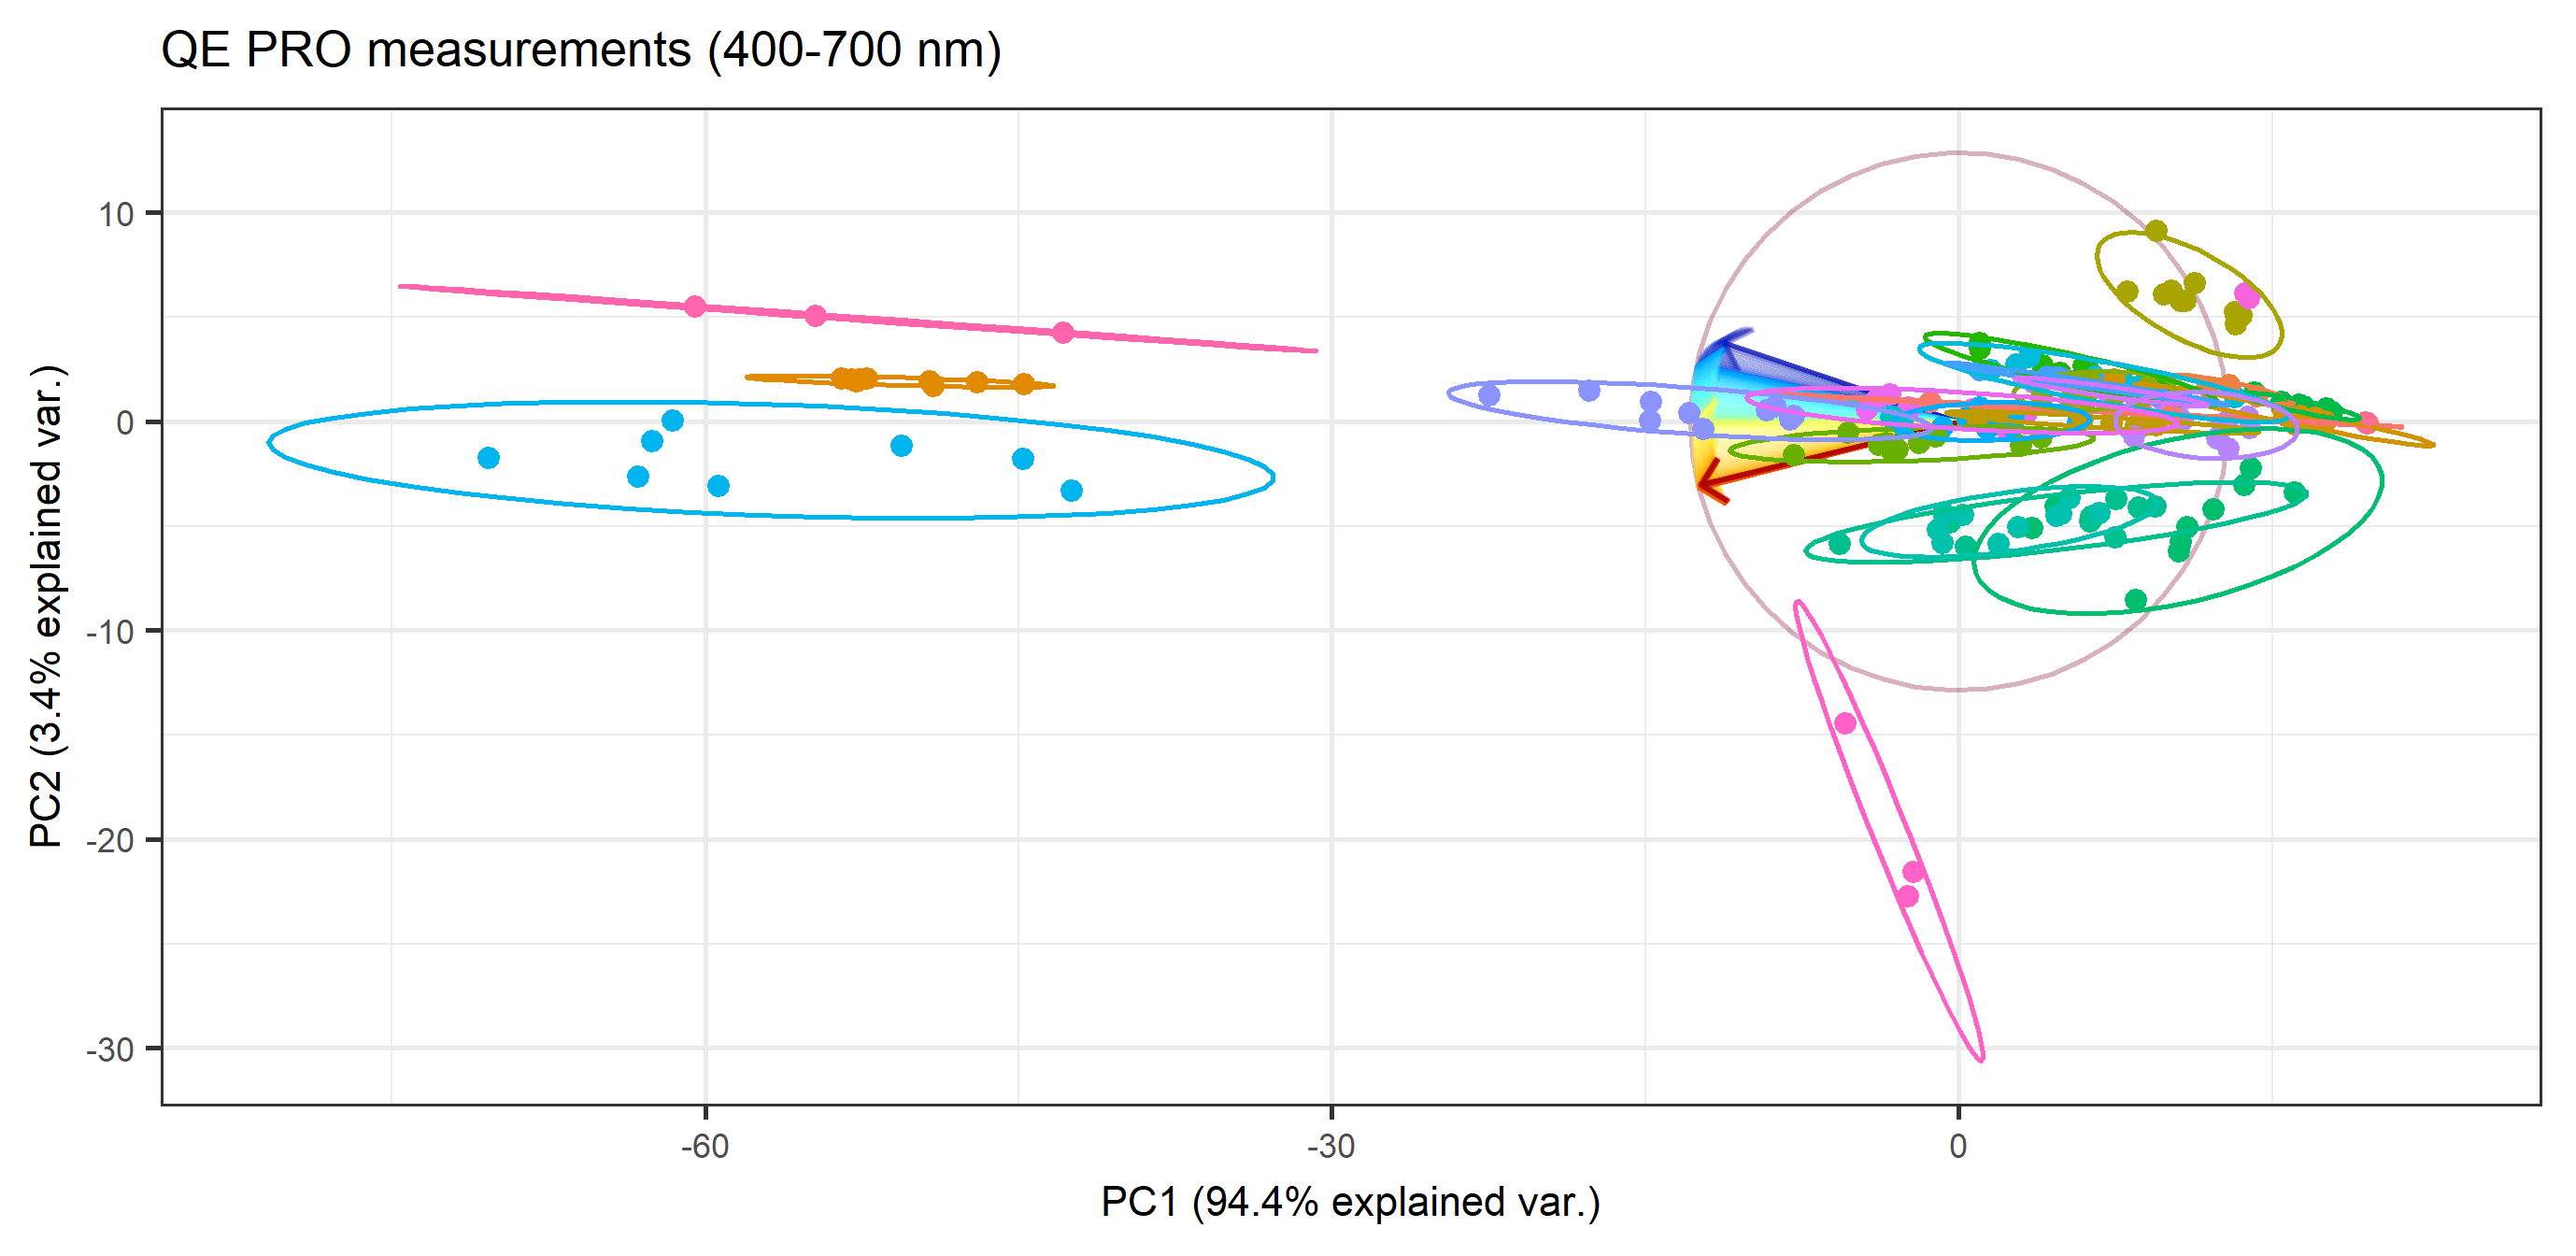
\includegraphics[width=1\textwidth]{Images/results/PCA_plastics_full_only_scat.png}
    \caption{Scatter plot of the results of the PCA with all plastic samples}
    \label{fig:PCA_plastics_only_full_scat}
\end{figure}


\begin{figure}[H]
   \centering
    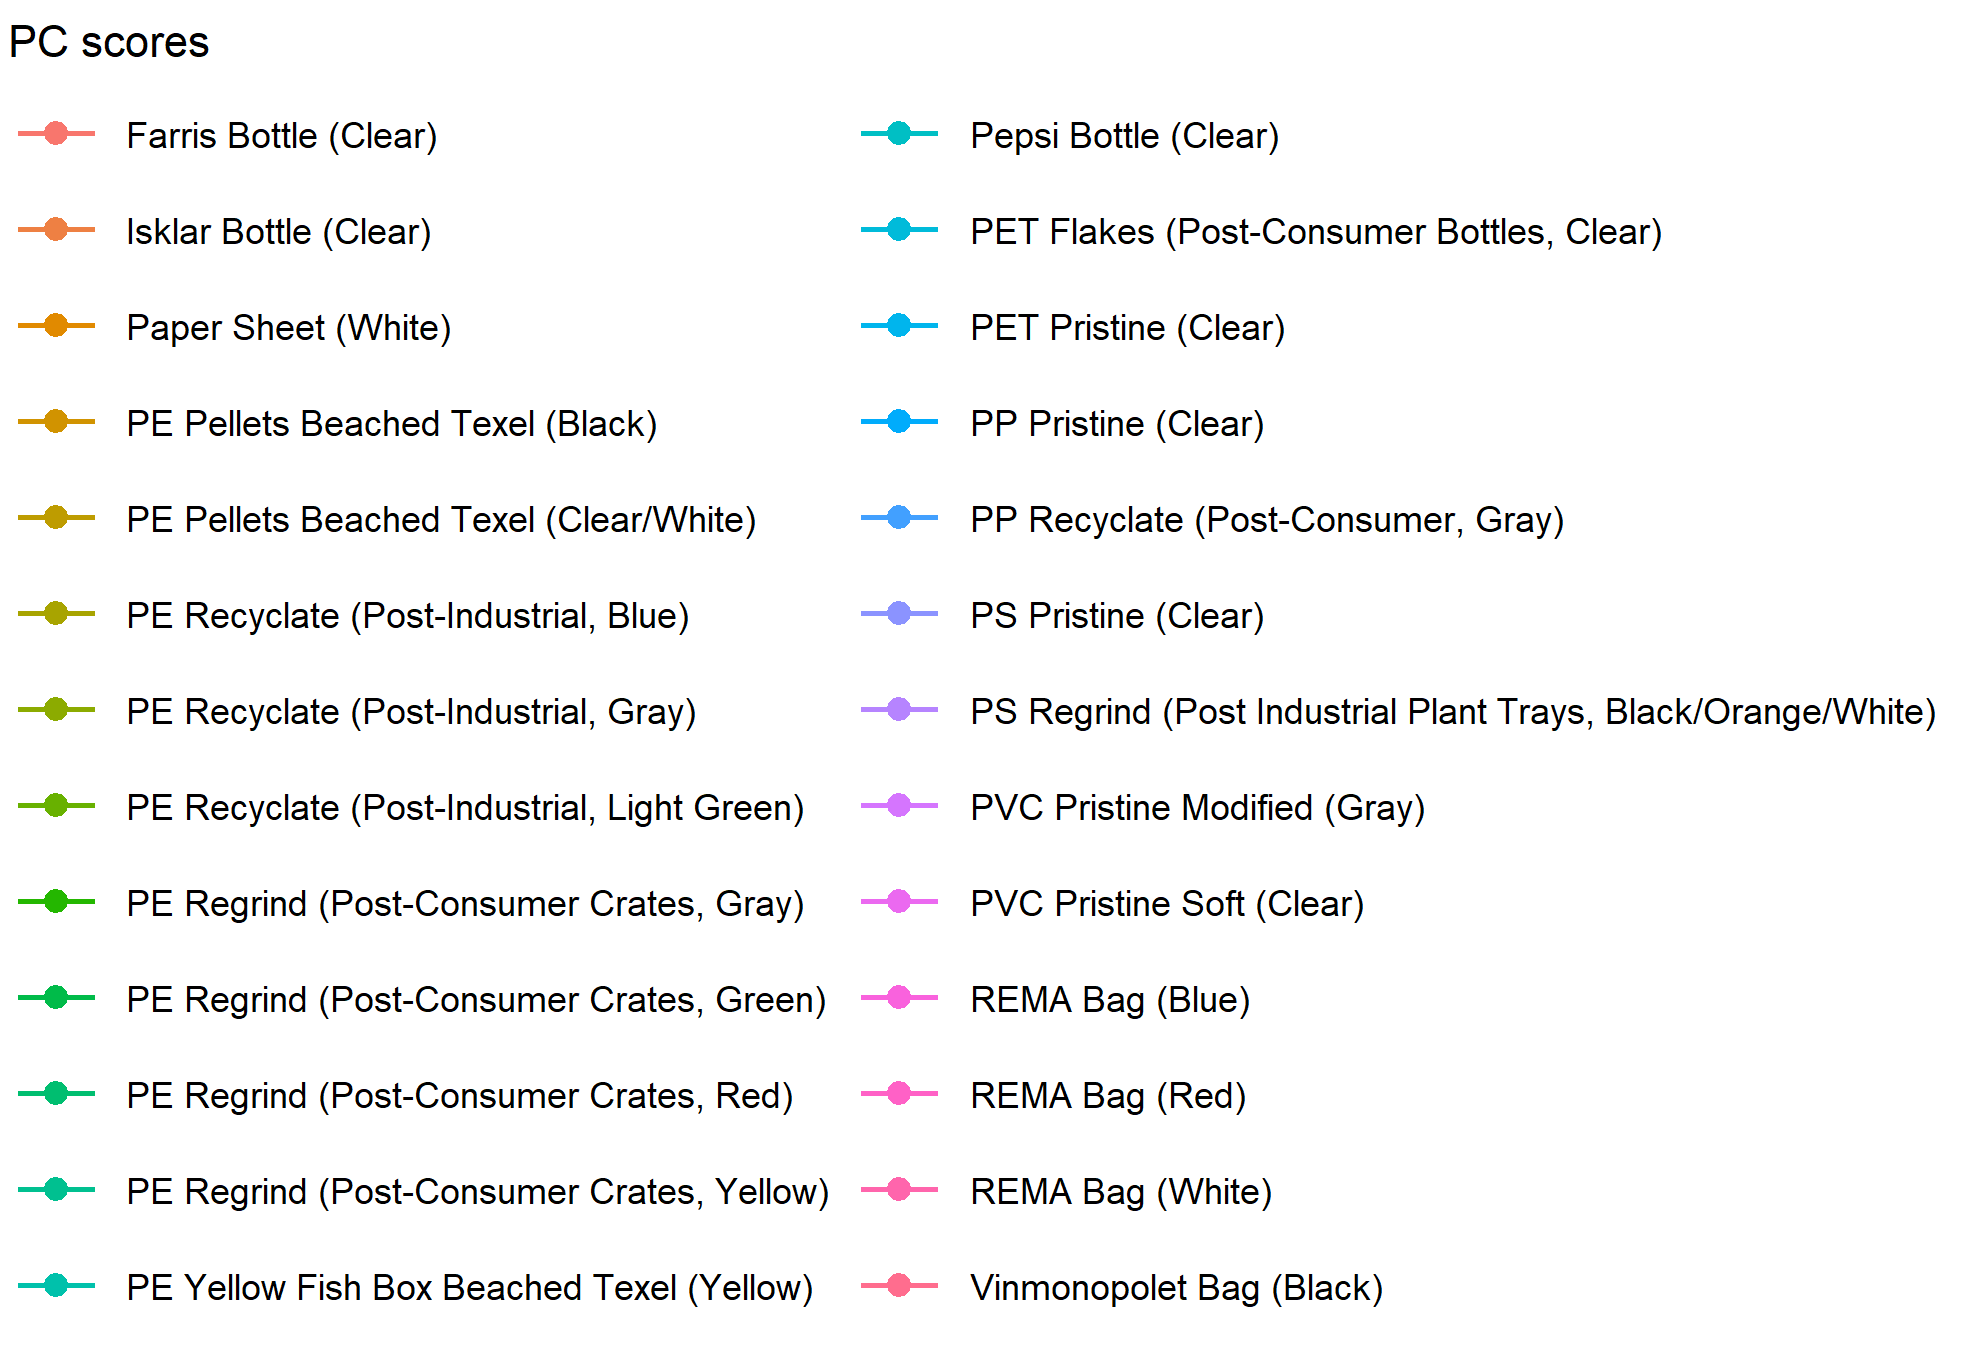
\includegraphics[width=0.7\textwidth]{Images/results/PCA_plastics_full_list.png}
  \caption{List of all scanned plastic samples and their respective colors.}
  \label{fig:PCA_plastics_full_list}
\end{figure}

\begin{figure}[H]
    \centering
    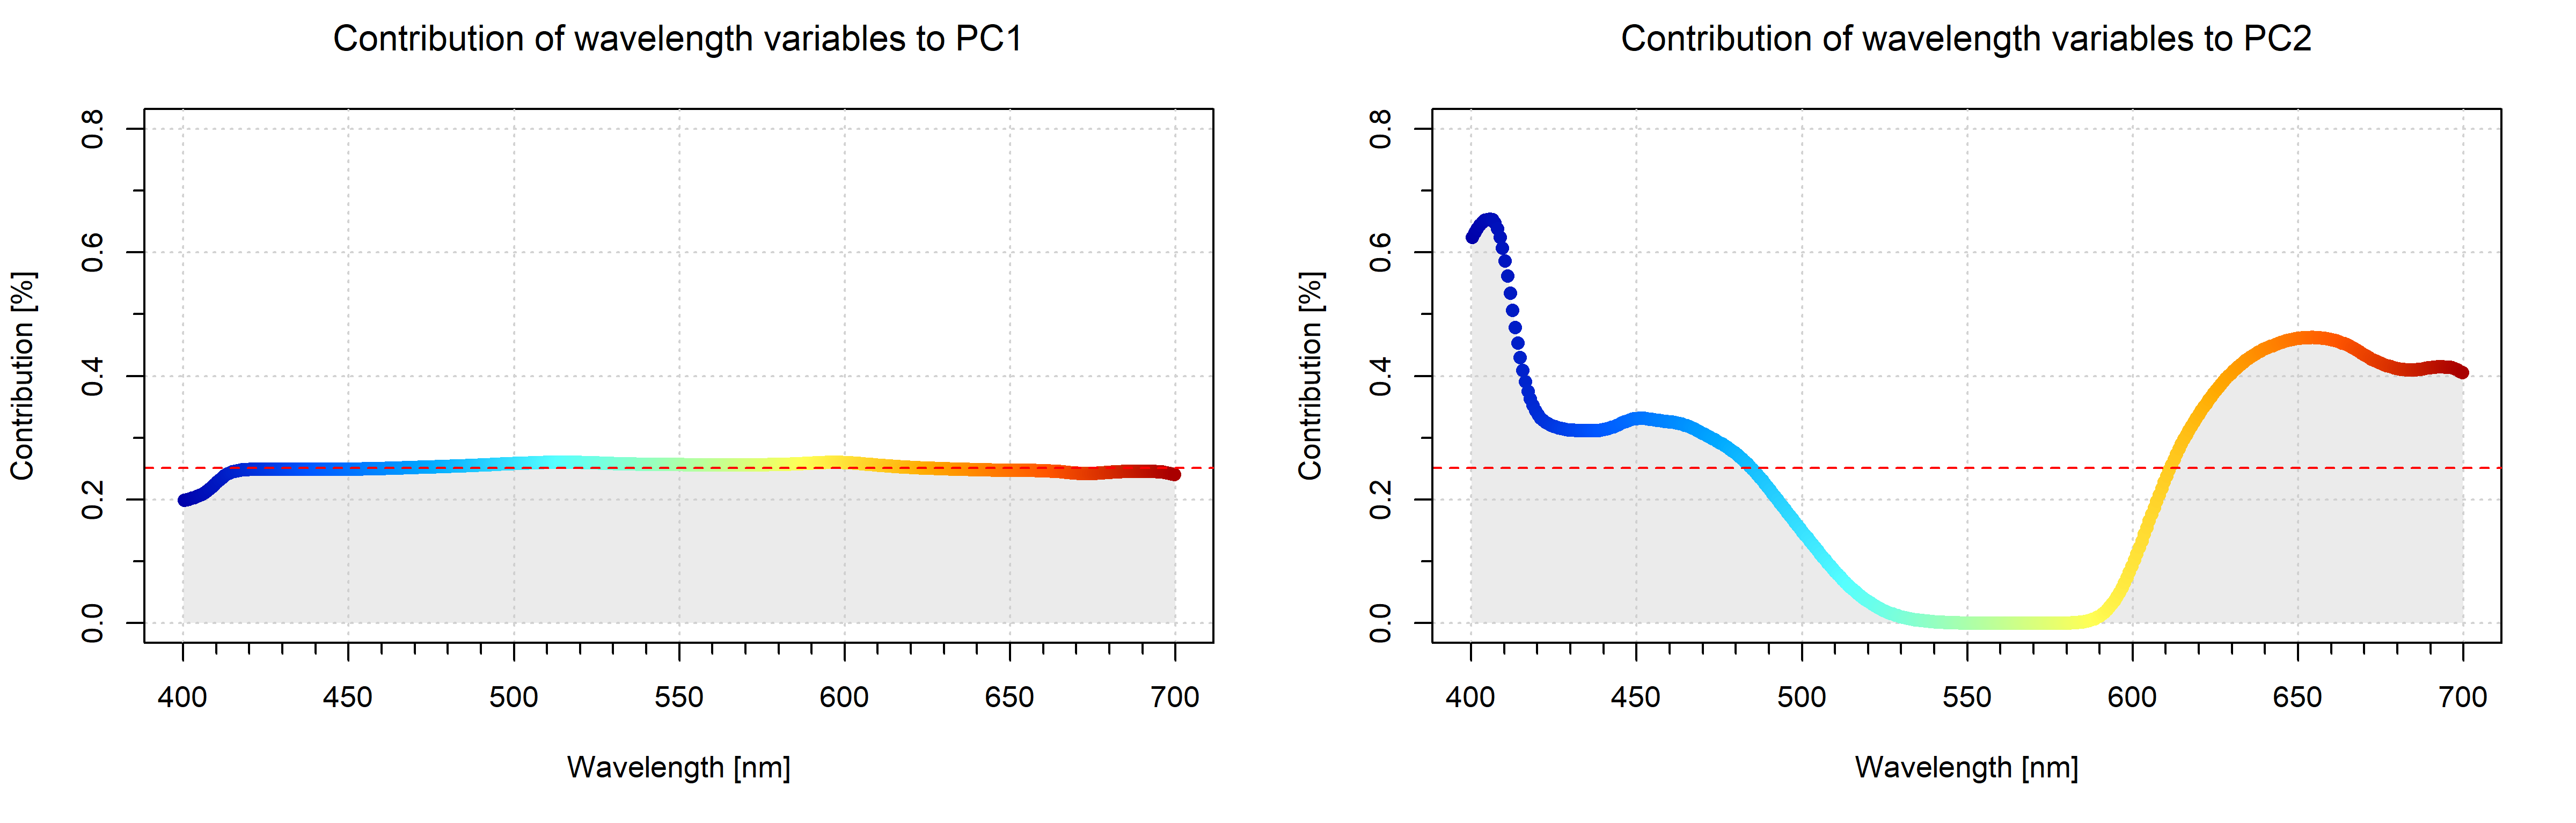
\includegraphics[width=1\textwidth]{Images/results/PCA_plastics_full_doub_cont.png}
    \caption{Contribution plot of the results of the PCA with all plastic samples.}
    \label{fig:PCA_plastics_full_doub_cont}
\end{figure}

\subsection{PCA with Reduced Plastic Samples}
However, despite the lower explanation percentage of PC2, there are clusters. These are quite apparent in the top and bottom of the scatter plot in figure \ref{fig:PCA_plastics_reduced_only_scat}. The issue arise when comparing these clusters to their respective plastic type. There are no other clear clusters related to these types of plastic. The clear clusters these types are a part of are based on the color of the plastic and not inherent properties of the material. The bottom cluster consists of PE Recyclate of the color blue together with samples from the blue in the logo on a plastic bag. Similarly, the top cluster consists of PE Regrind and PE Yellow Fish Box Beached Texel, both of which are yellow in color. It is therefore difficult to argue that these clusters indicate anything other than the color additives in the material.
\\\\
%Tenke på å markere clusterene med tall, slik at det blir lettere å omtale
Based on the tendency of the clear plastic to be on the left side of the cluster, one can assume that the white paper background have had an impact on the results, and subsequently on the principal components. The samples of PS Pristine were particularly clear, as may be seen in the \textit{Materials} subsection of \textit{Methods}. Given that these are the main contributions to the spread along the horizontal axis, one could argue that without the light background, the lightness and clearness of the material would be less prominent in the first principal component. This would possibly further change the composition of the principal components and subsequently change the patterns on the scatter plots. 
\\\\%Snakke med Asgeir om dette og høre hva han tenker om at papiret har påvirket resultatene og at vi i utgangspunktet ikke har tid til å tilbringe en hel ny dag på laben for å teste på nytt. Aksel har gjort tester tidligere der han har fått samme resultat med at "lysheten" til prøvene har hatt stor innvirkning
\todo[inline, color = orange!40]{burde avsnittene over heller være i discussion}
\noindent
The contribution plot of the second principal component does show that the lower end of the spectrum has ha larger impact than the larger wavelengths. 

\begin{figure}[H]
    \centering
    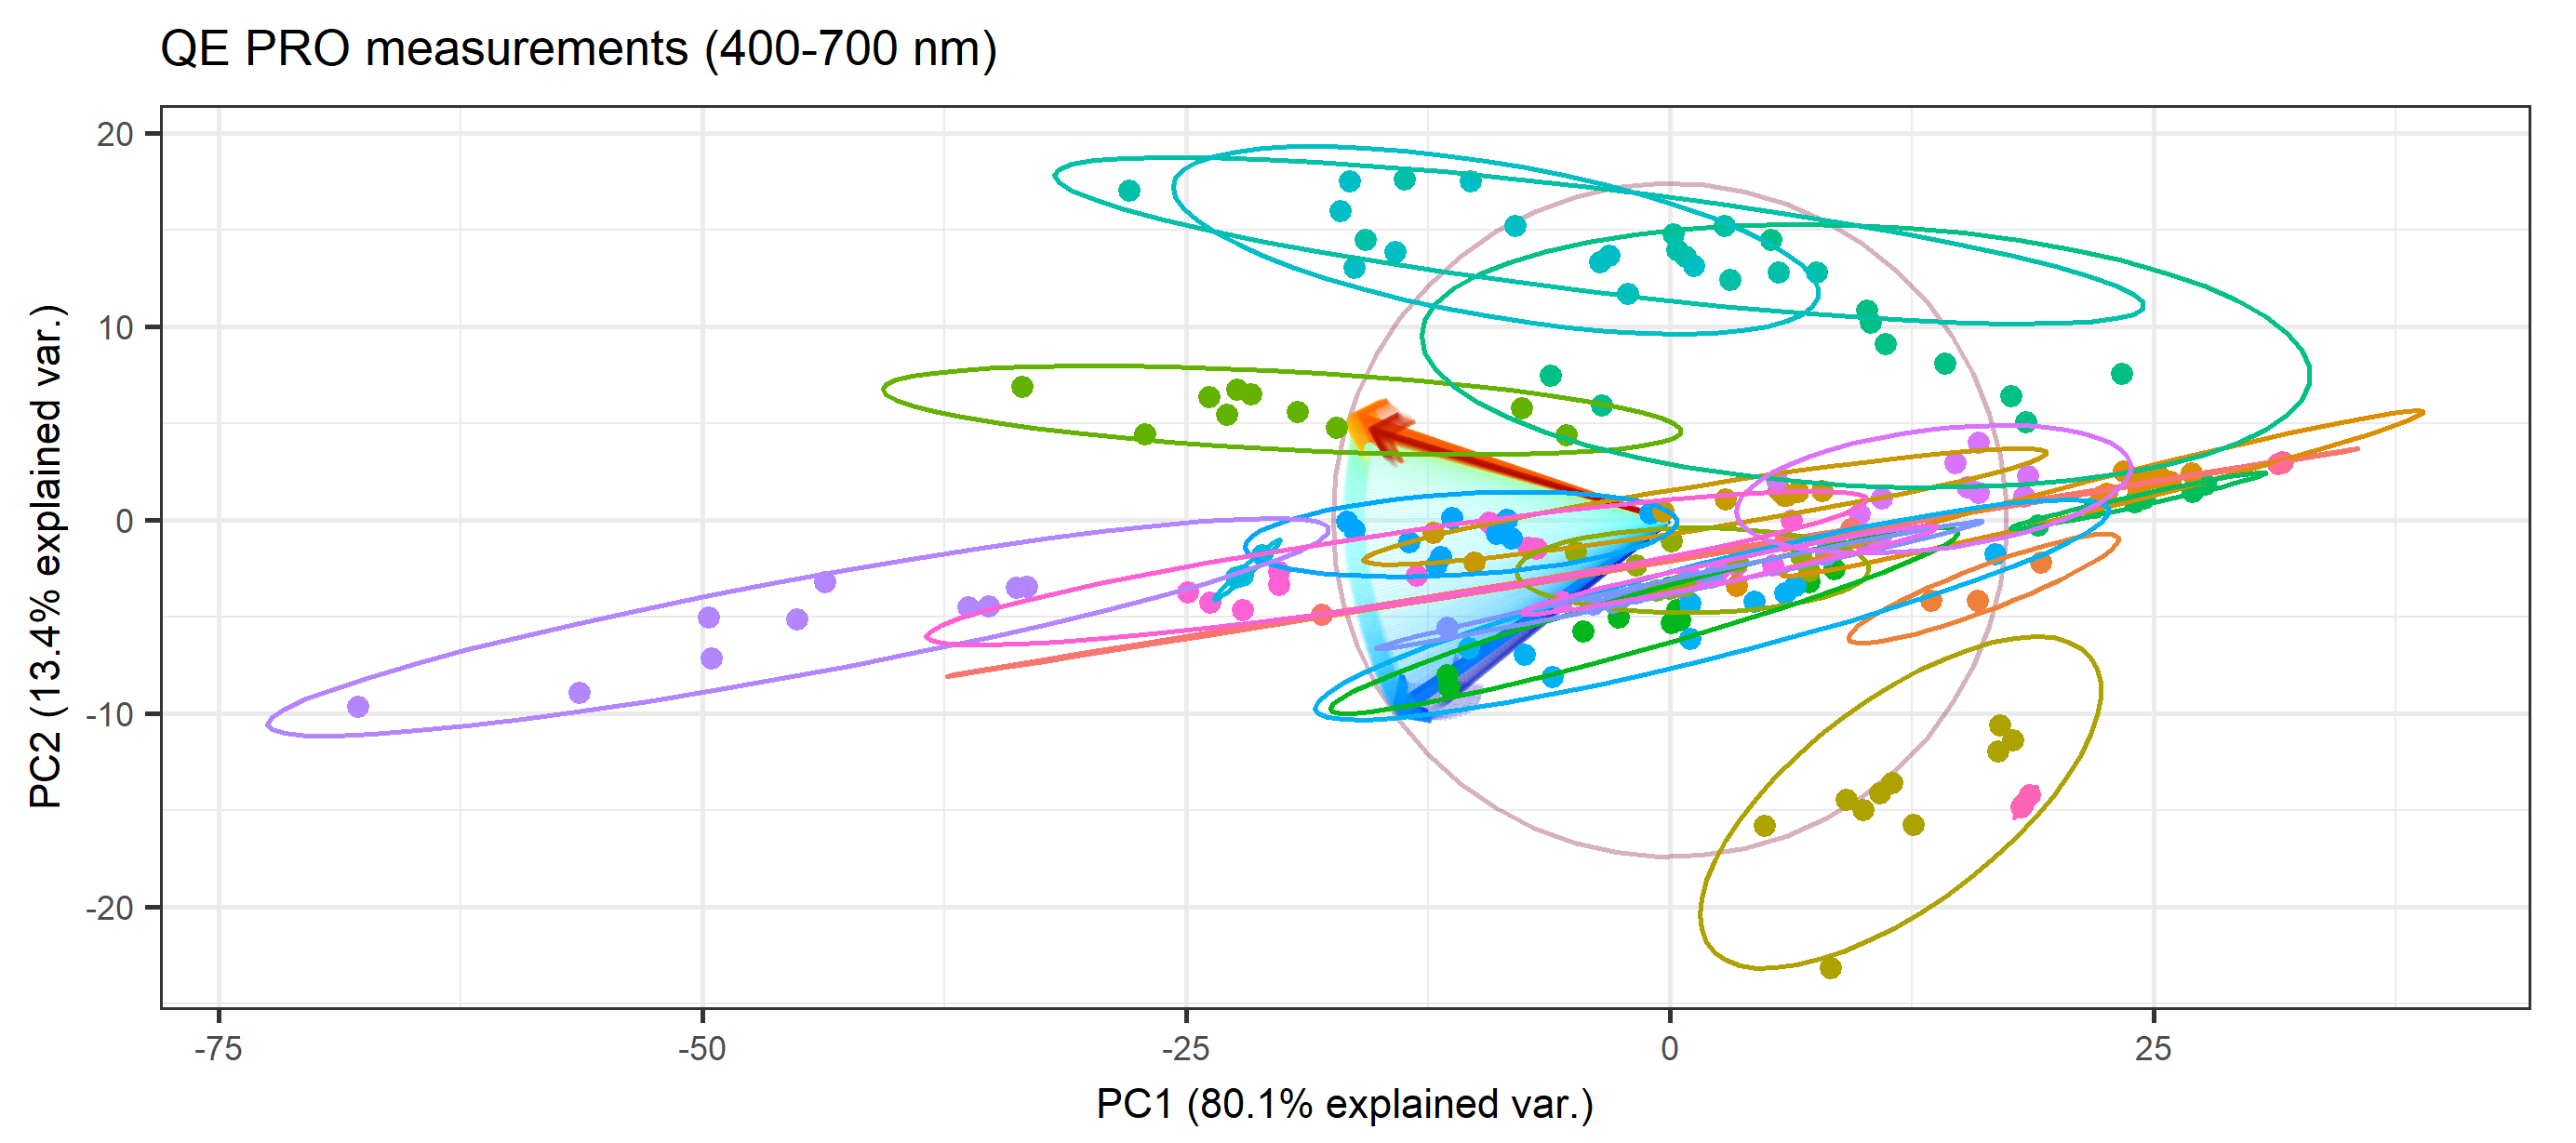
\includegraphics[width=1\textwidth]{Images/results/PCA_plastics_reduced_only_scat.png}
    \caption{Results of the PCA with reduced Plastic Samples}
    \label{fig:PCA_plastics_reduced_only_scat}
\end{figure}

\begin{figure}[H]
    \centering
    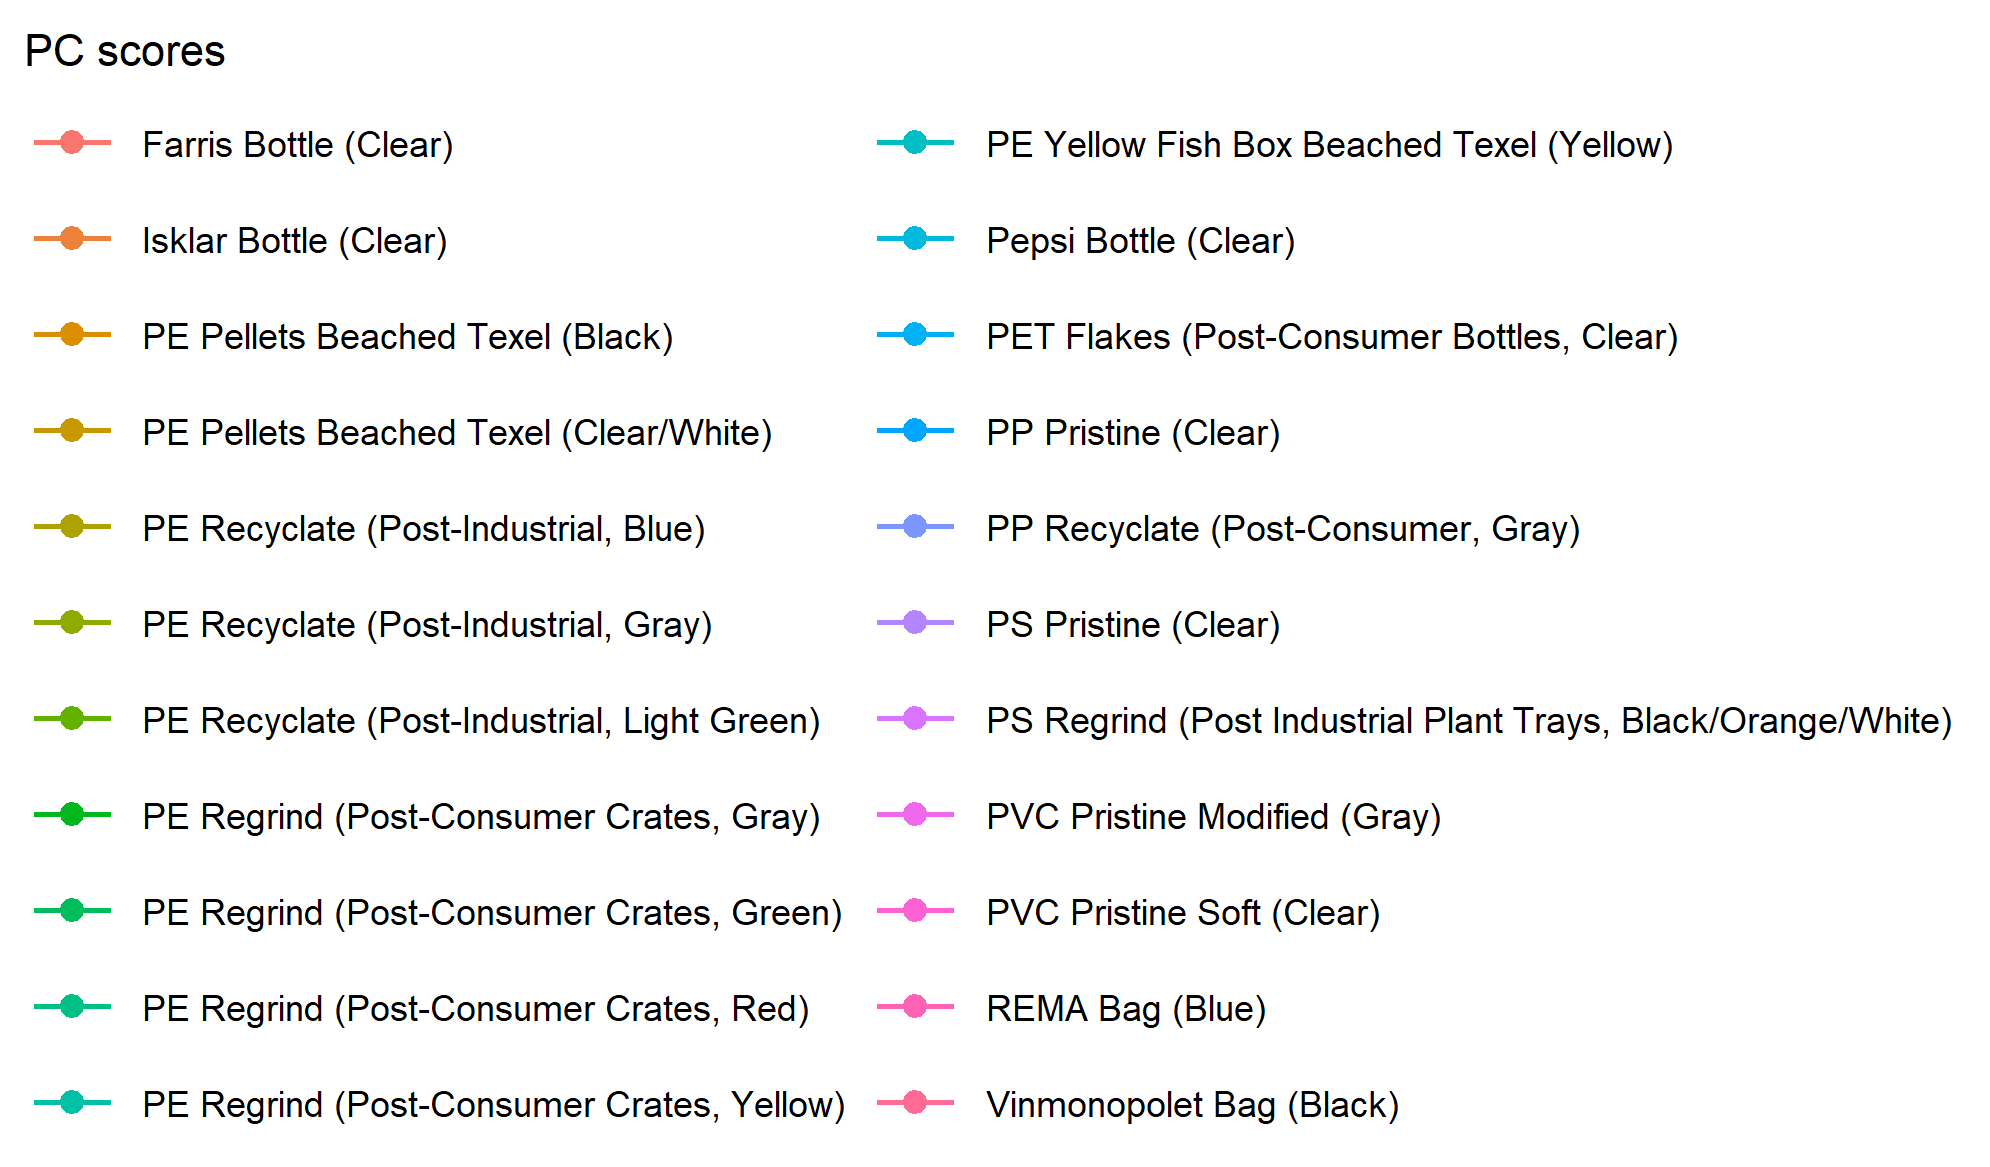
\includegraphics[width=0.7\textwidth]{Images/results/PCA_plastics_reduced_list.png}
    \caption{List of the reduced scanned plastic samples and their respective colors.}
    \label{fig:PCA_plastics_reduced_list}
\end{figure}

\begin{figure}[H]
    \centering
    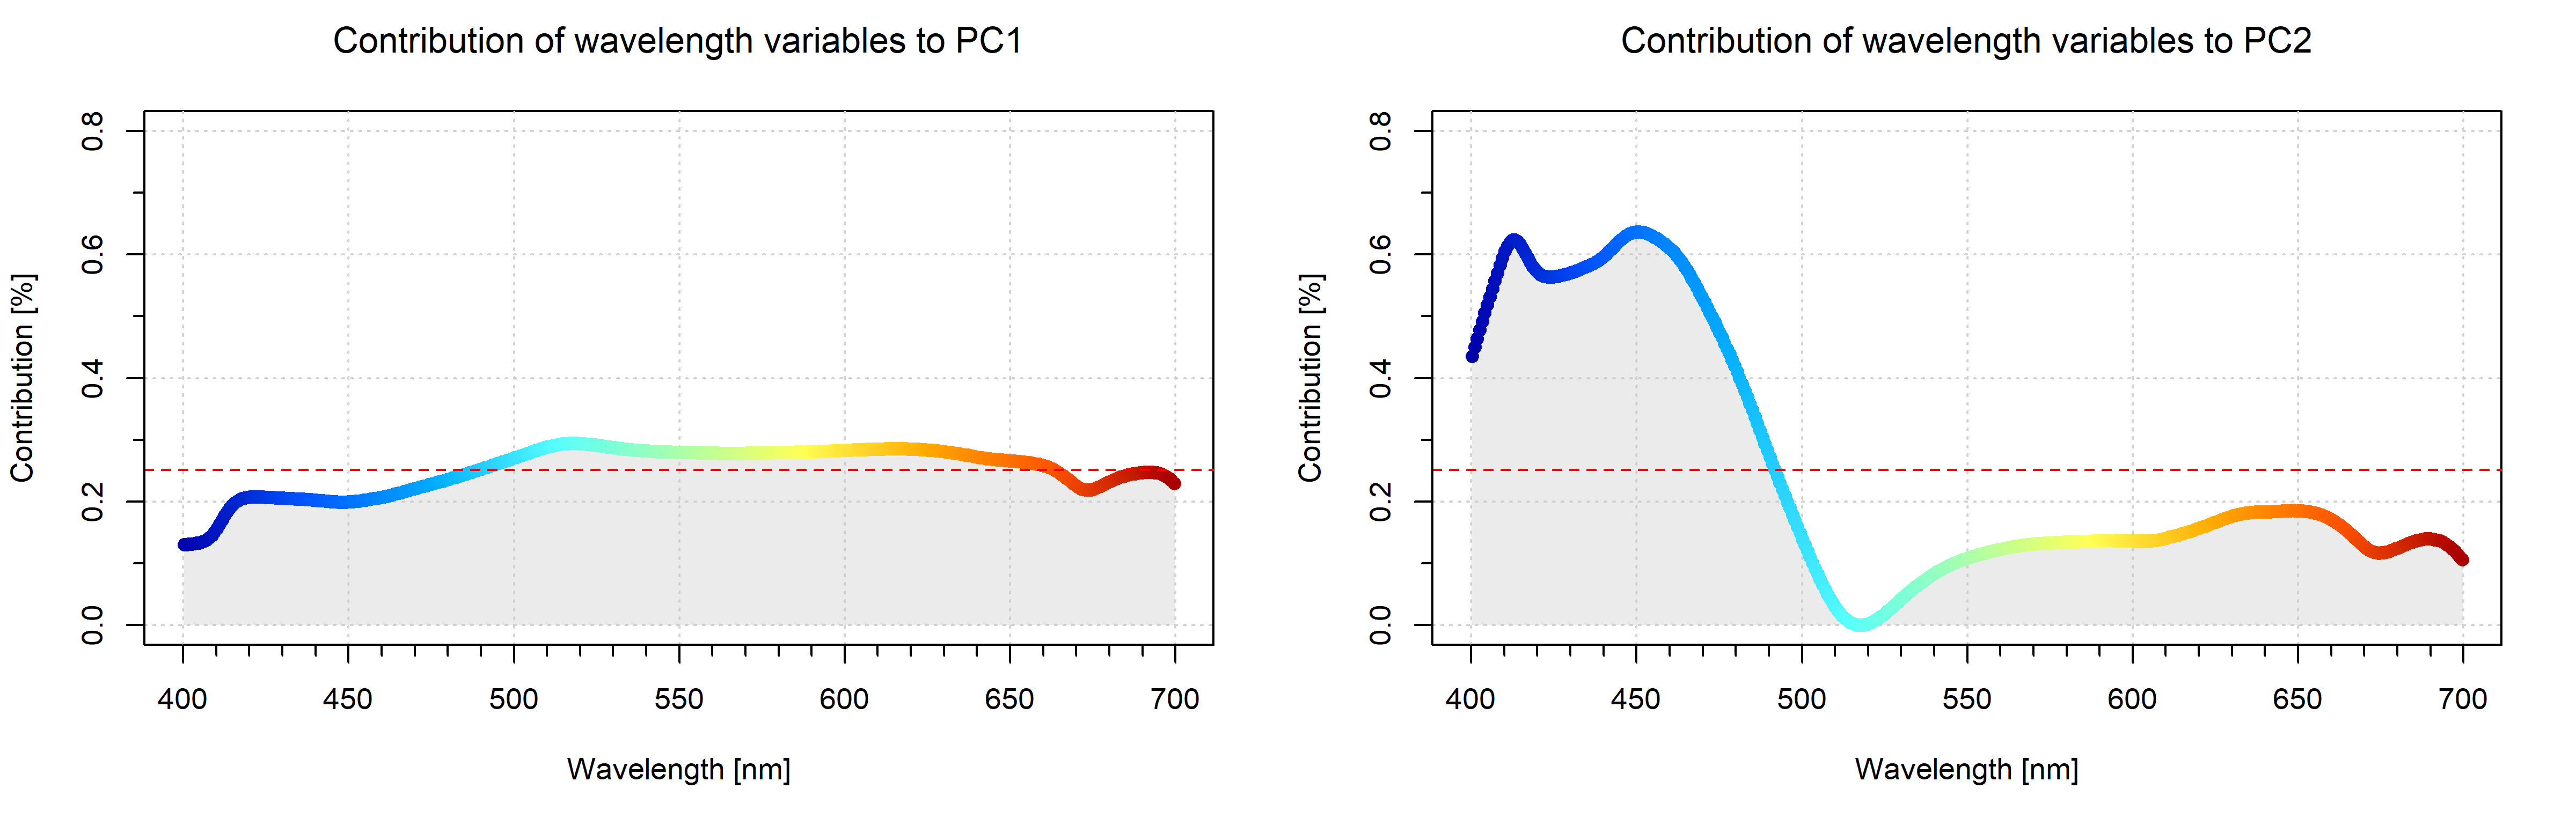
\includegraphics[width=1\textwidth]{Images/results/PCA_plastics_reduced_doub_cont.png}
    \caption{Contribution plots of the two principal components of the PCA with reduced plastic samples}
    \label{fig:PCA_plastics_doub_cont}
\end{figure}

\subsection{PCA with Biological Components}
When compared to results from testing on biological pigments, a more prominent trend became apparent. The natural occurring pigment in algae and crustaceans differed from the plastic in the scatter plot. This shows potential for distinguishing plastic in general from organic pigments naturally occurring in the marine environment.
\\\\%Argumentere med at her ser man at den klare plasten ligger utenfor konfidens intervallet og kan dermed mulig ekskluderes i en ny runde med forsøk, eventuelt at man endre bakgrunnen slik at den ikke er hvit og dermed ikke påvirker lysheten i tilsvarende grad. 
Below are plots with the same composition as those which solely contain plastic. The contribution on the first principal component does not differ much from that in the previous plots. However, given the mentioned effect of the clear plastic, this might change with the use of a less reflective background. Furthermore, in figure \ref{fig:PCA_plastics_and_biology_scat} all plastic samples are gathered in one confidence interval ring. The clear result is that the previously mentioned clear plastic lies outside the confidence interval. This would further underline the previous suspicion that there is a prominent effect from the white background on the results.
\\\\
Experience has shown that the brightness/lightness of the samples is highly relevant also when not investigating plastic. Therefore, the change in background might affect the results, but it is not expected to revolutionize them.

\begin{figure}[H]
    \centering
    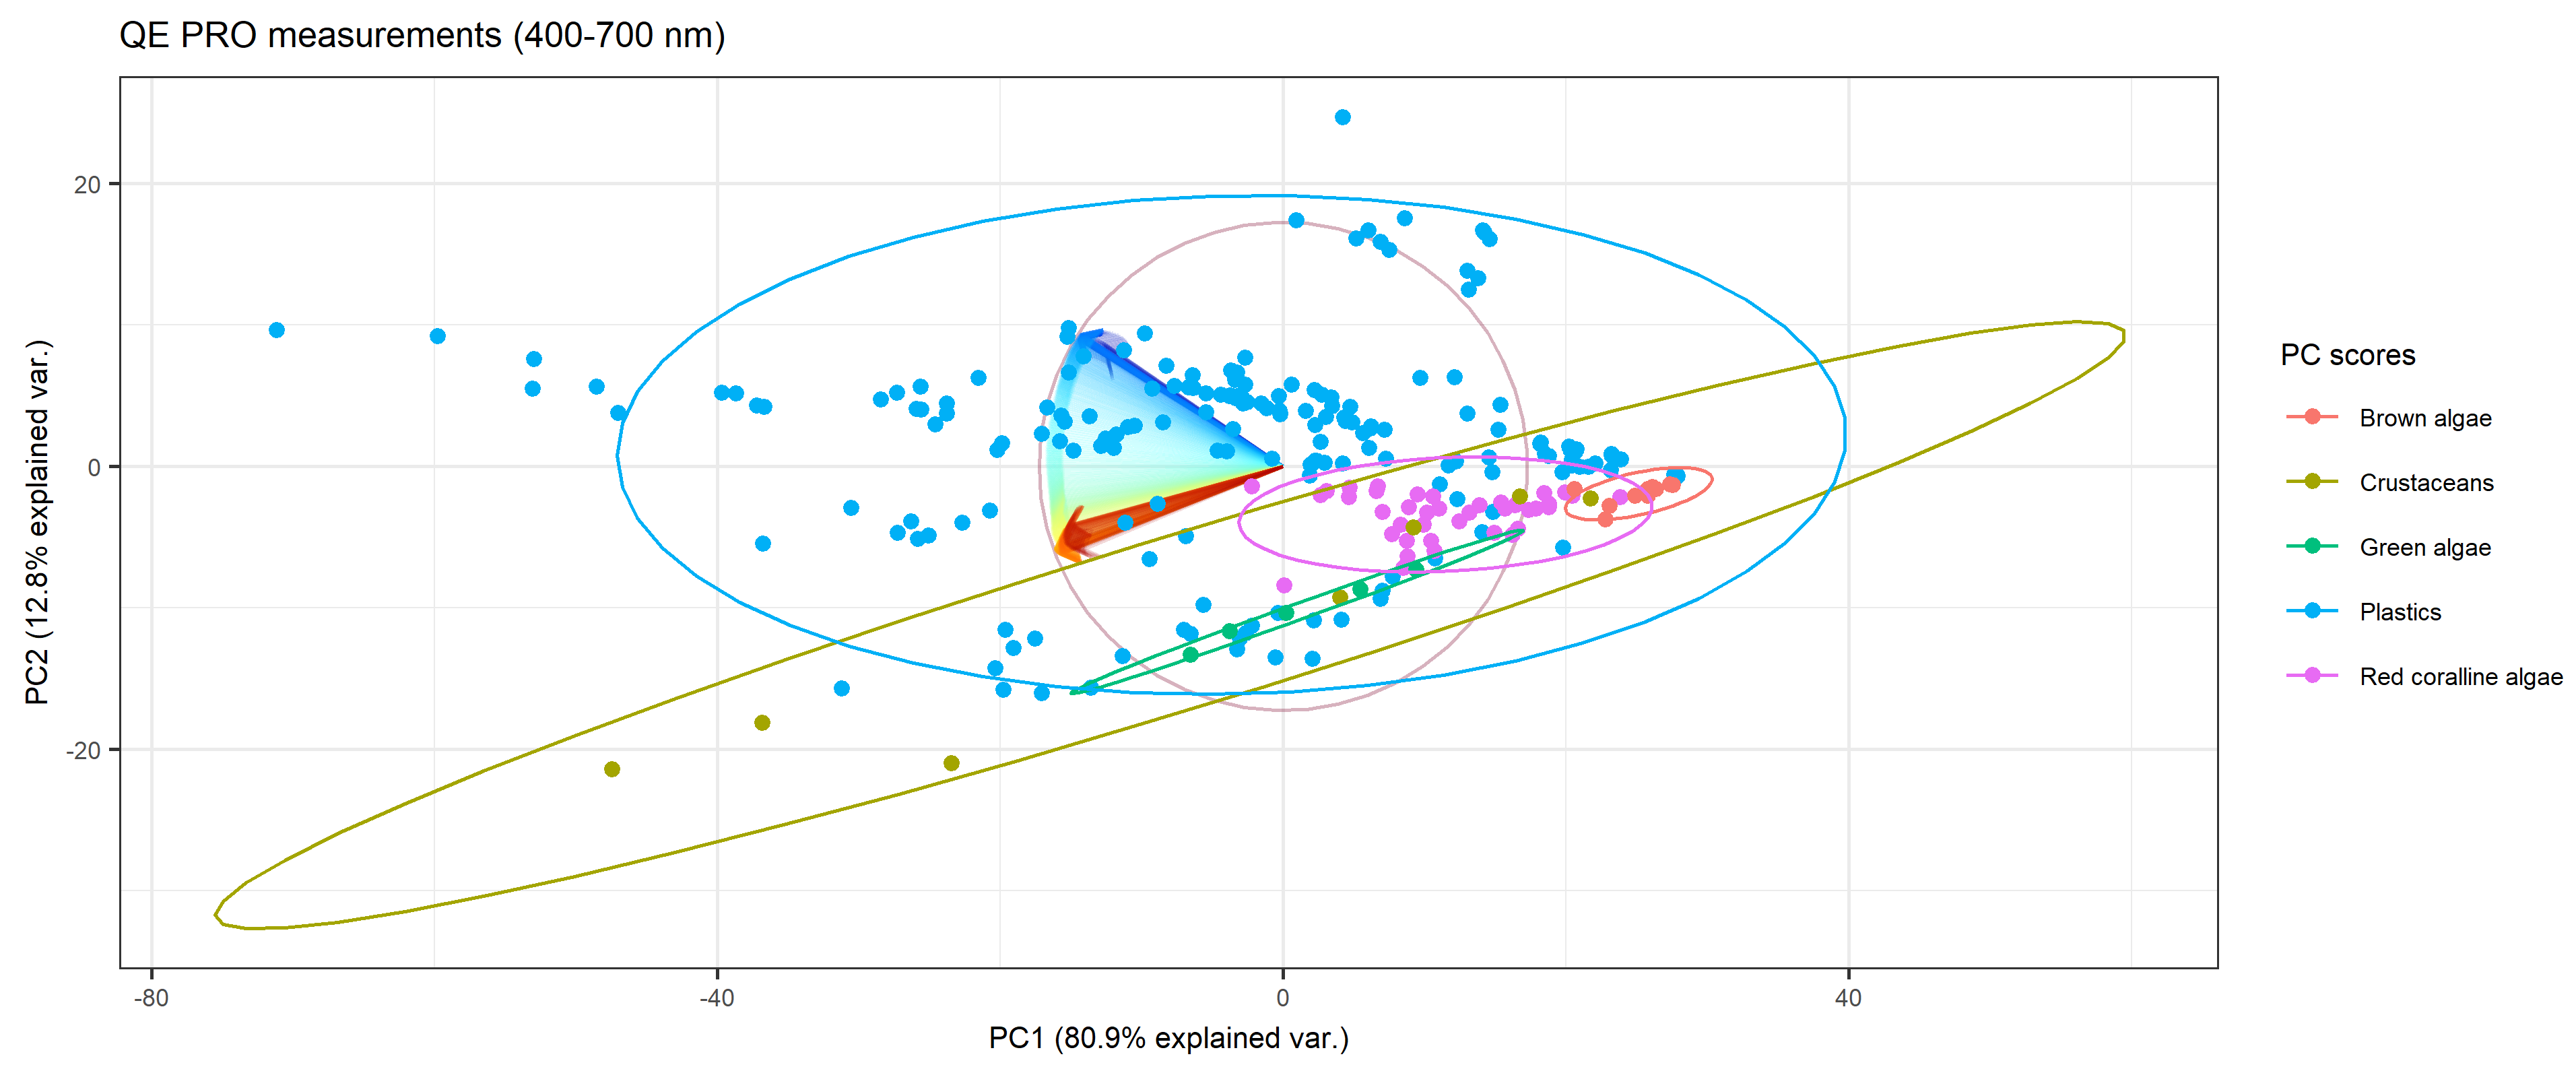
\includegraphics[width=1\textwidth]{Images/results/PCA_plastics_and_biology_scat_clust.png}
    \caption{Results of the PCA with Plastics and Biological Components}
    \label{fig:PCA_plastics_and_biology_scat}
\end{figure}


\begin{figure}[H]
  \newcommand*\FigVSkip{0.5em}
  \newcommand*\FigHSkip{0.1em}
  \newsavebox\FigBox
  \centering
  % Top image is centered, so no need to get width
 \sbox{\FigBox}{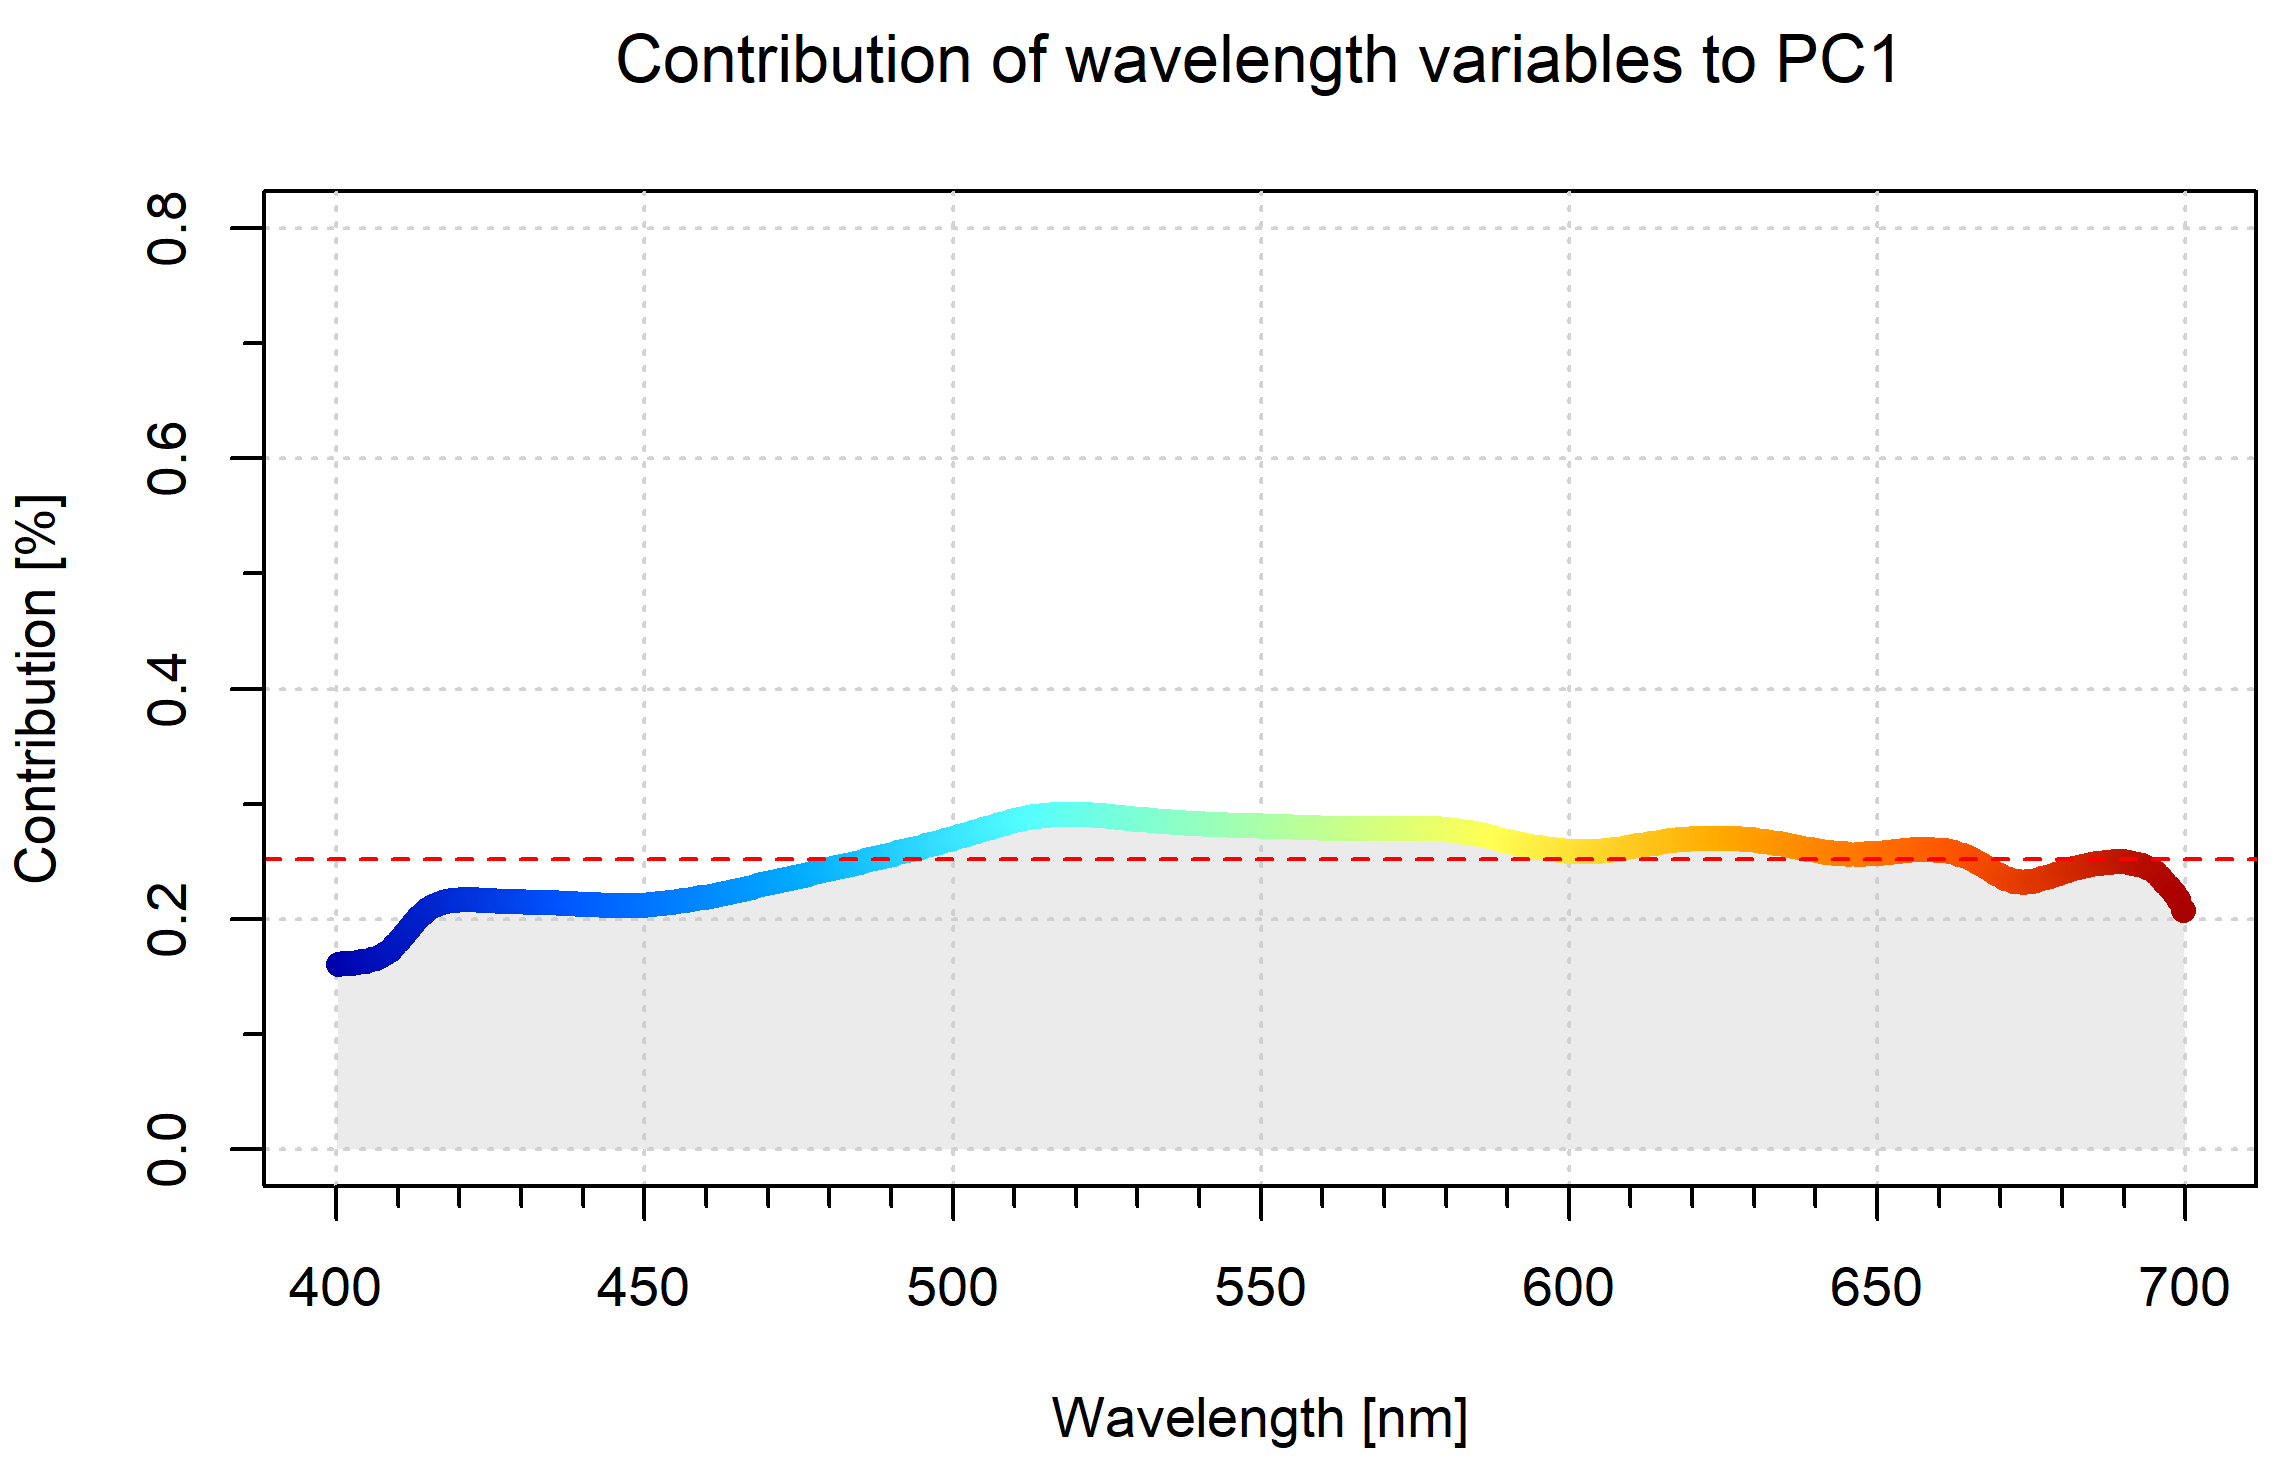
\includegraphics[scale=0.5]{Images/results/PCA_plastics_and_biology_cont_pc1.png}}
  \begin{minipage}{\wd\FigBox}
    \centering\usebox{\FigBox}
     \label{fig:PCA_plastics_and_biology_cont_pc1}
  \end{minipage}
    % Top image is centered, so no need to get width
 \sbox{\FigBox}{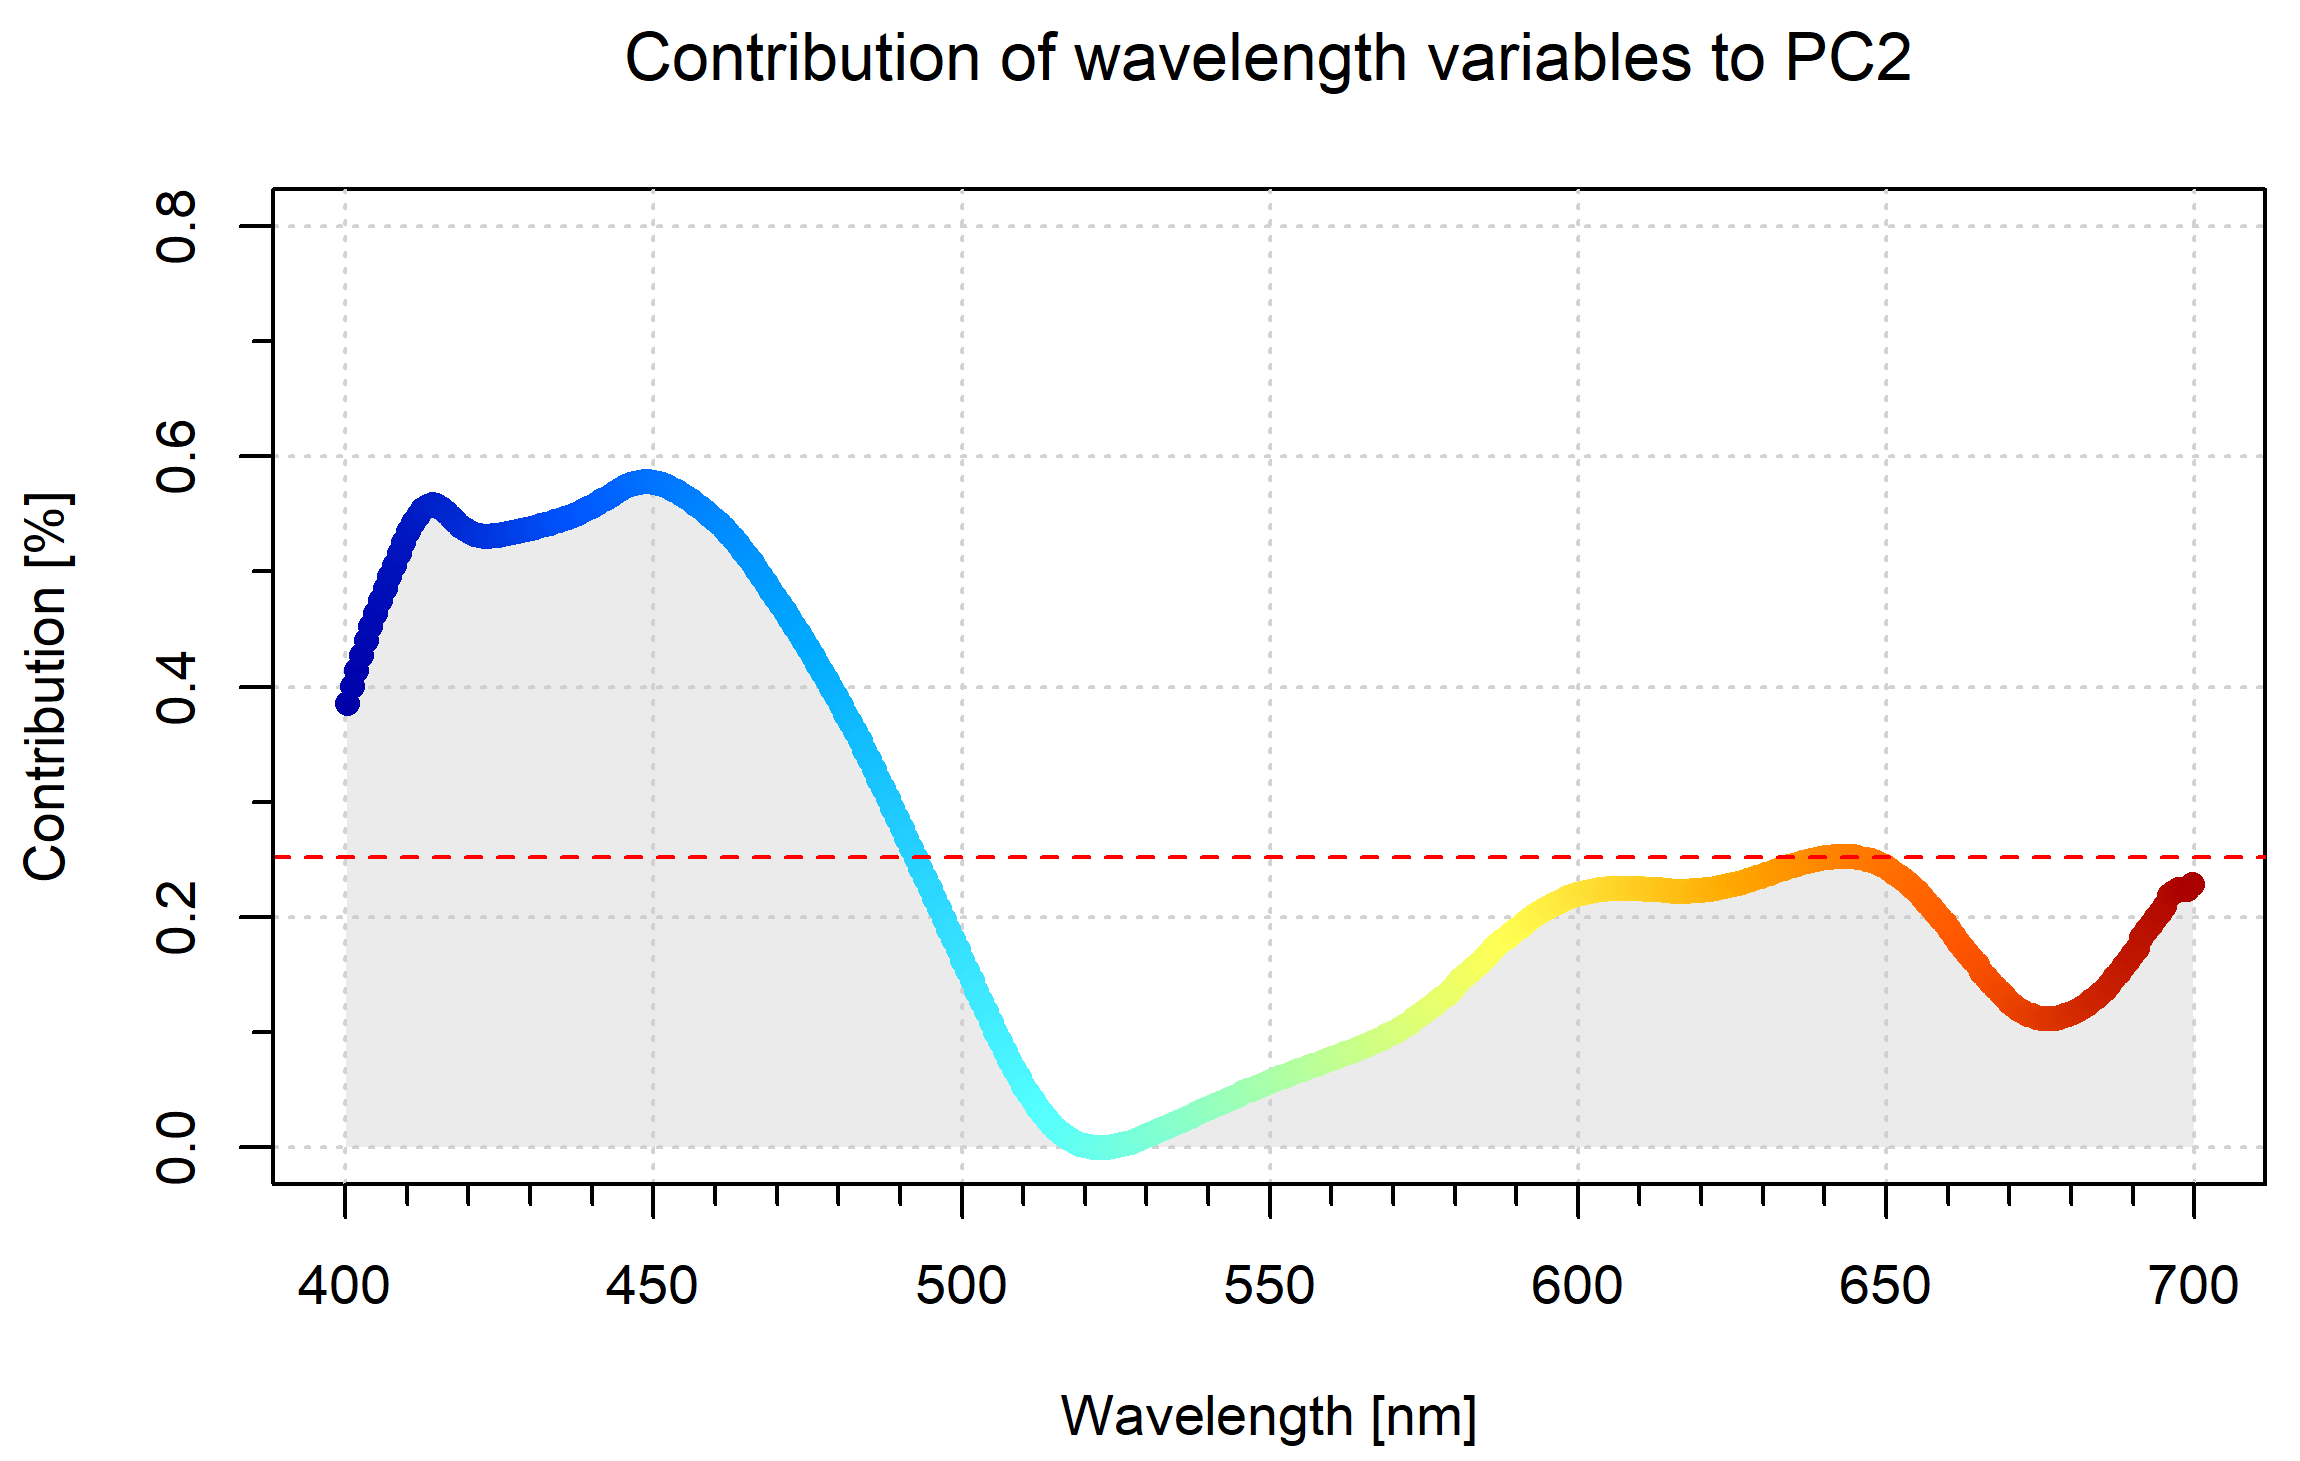
\includegraphics[scale=0.5]{Images/results/PCA_plastics_and_biology_cont_pc2.png}}
  \begin{minipage}{\wd\FigBox}
    \centering\usebox{\FigBox}
  \label{fig:PCA_plastics_and_biology_cont_pc2}
  \end{minipage}
  % Save second image 
  \caption{Contribution plots for the PCA with plastic and biological samples}
\label{fig:PCA_and_bio_cont_plots}
\end{figure}


\vspace{1.3cm}
\section{Signatures}

\subsection{Constant Color}
The resulting signatures were highly affected by the color of the targeted plastic pellets. The figure below, Figure \ref{fig:plastcomp1}, shows the spectrum of two types, PP and PVC respectively. 

\begin{figure}[H]
  \newcommand*\FigVSkip{0.5em}
  \newcommand*\FigHSkip{0.1em}
  \newsavebox\FigBox
  \centering
  % Top image is centered, so no need to get width
 \sbox{\FigBox}{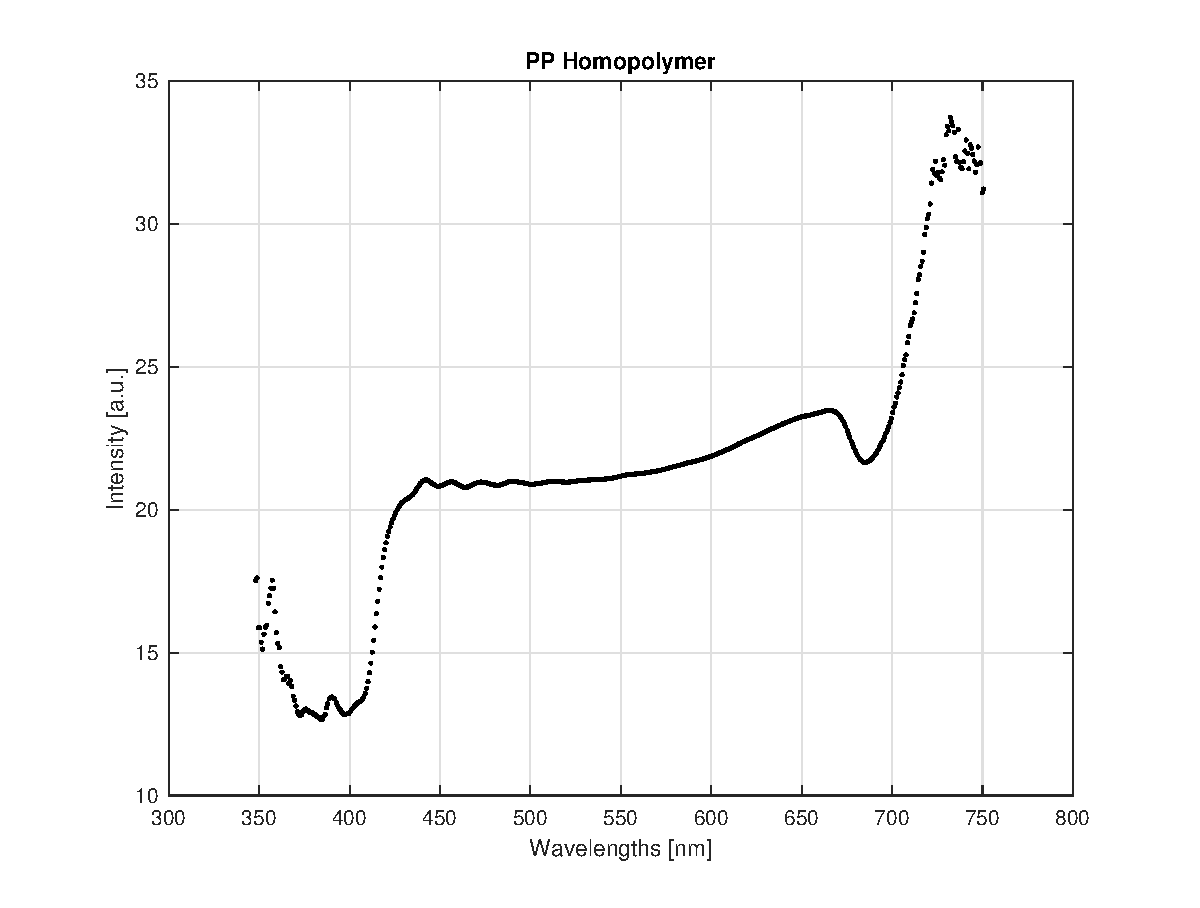
\includegraphics[scale=0.36]{Images/appendix/pp-pristine-clear.eps}}
  \begin{minipage}{\wd\FigBox}
    \centering\usebox{\FigBox}
    \subcaption{a) PP Pristine}
  \end{minipage}
    % Top image is centered, so no need to get width
 \sbox{\FigBox}{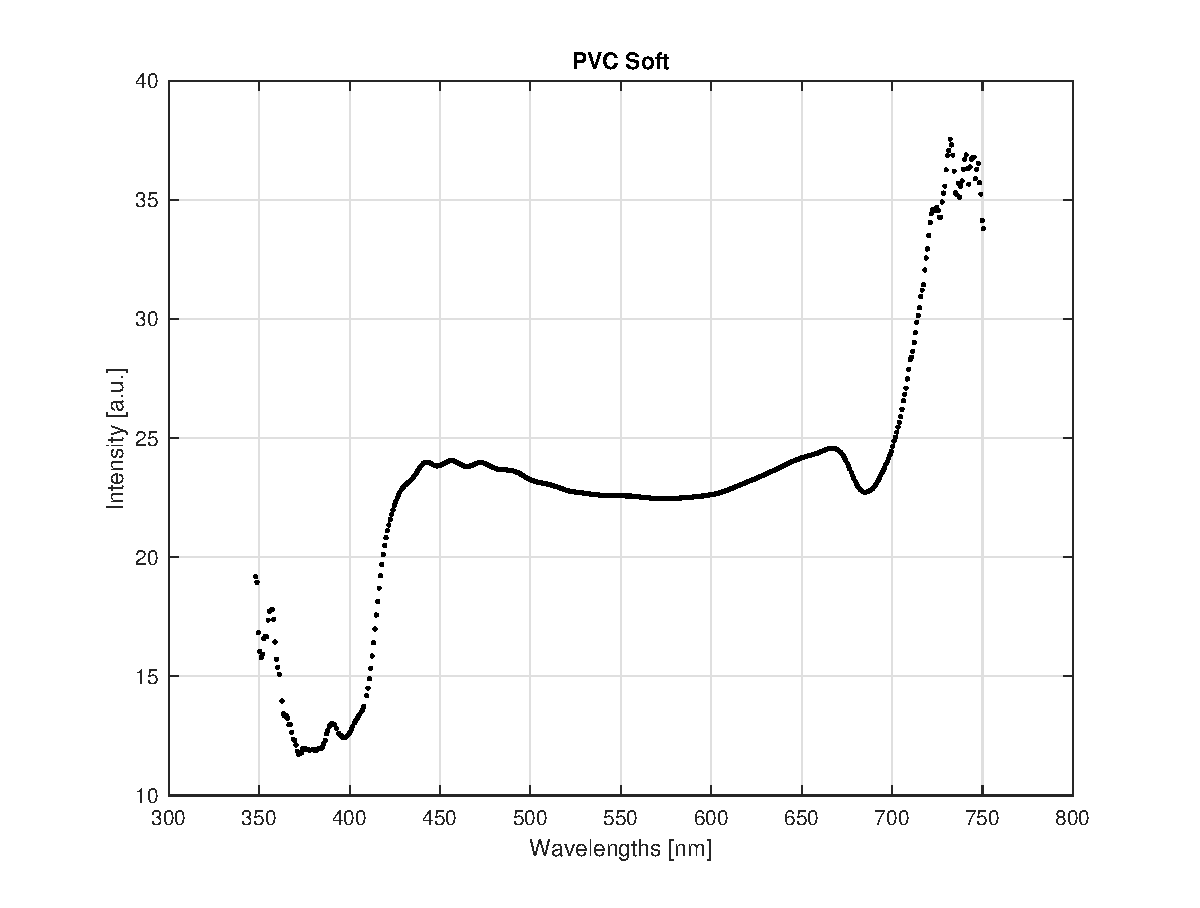
\includegraphics[scale=0.36]{Images/appendix/pvc-soft-pristine-clear.eps}}
  \begin{minipage}{\wd\FigBox}
    \centering\usebox{\FigBox}
    \subcaption{b) PVC Soft Pristine}
  \end{minipage}
  % Save second image 
  \caption{A comparison of the resulting signature for PP and PVC - both clear-colored}
  \label{fig:plastcomp1}
\end{figure}

%denne viser gule for pe og pe-hd, men de er kanskje for like..
\begin{comment}
\begin{figure}[H]
  \newcommand*\FigVSkip{0.5em}
  \newcommand*\FigHSkip{0.1em}
  \newsavebox\FigBox
  \centering
  % Top image is centered, so no need to get width
 \sbox{\FigBox}{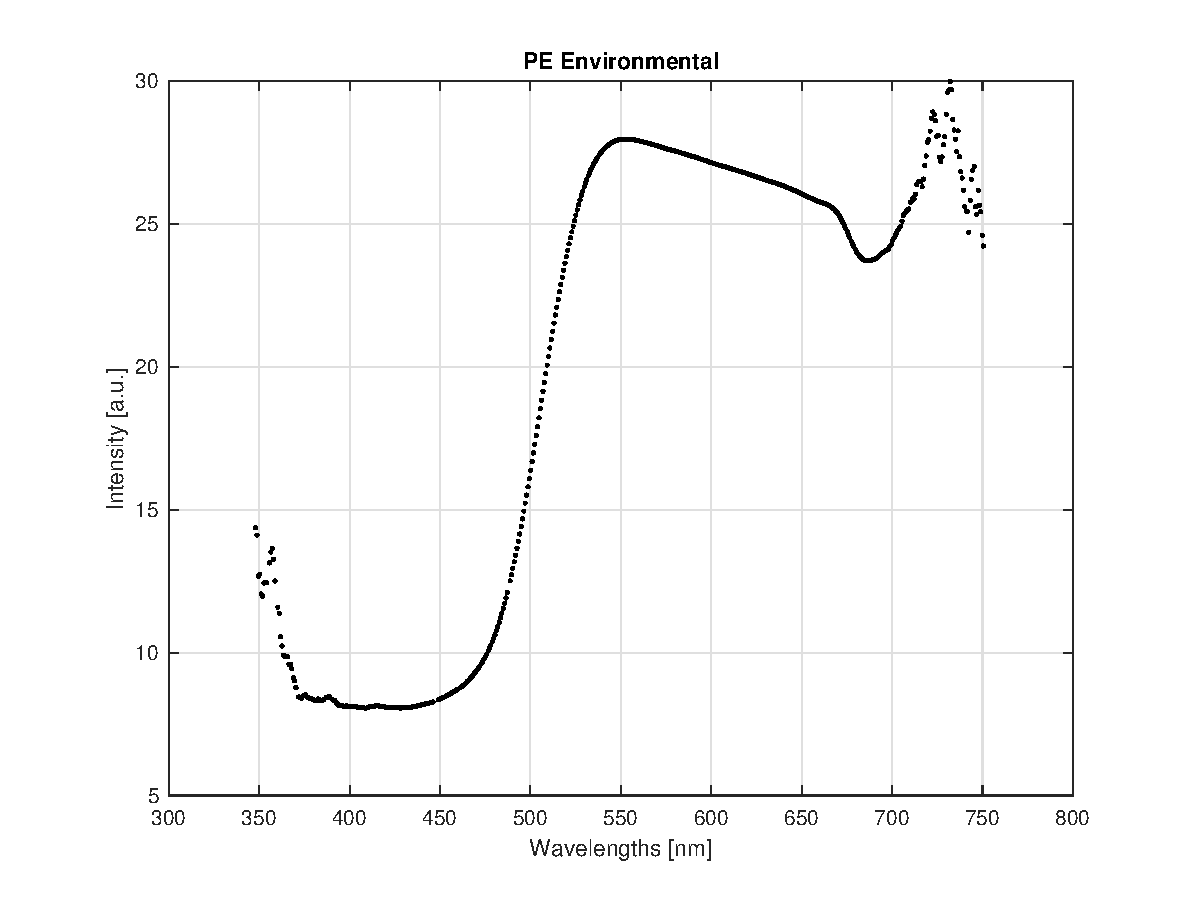
\includegraphics[scale=0.36]{Images/appendix/p-env_yellowbowl.eps}}
  \begin{minipage}{\wd\FigBox}
    \centering\usebox{\FigBox}
    \subcaption{a) PE Environment}
  \end{minipage}
    % Top image is centered, so no need to get width
 \sbox{\FigBox}{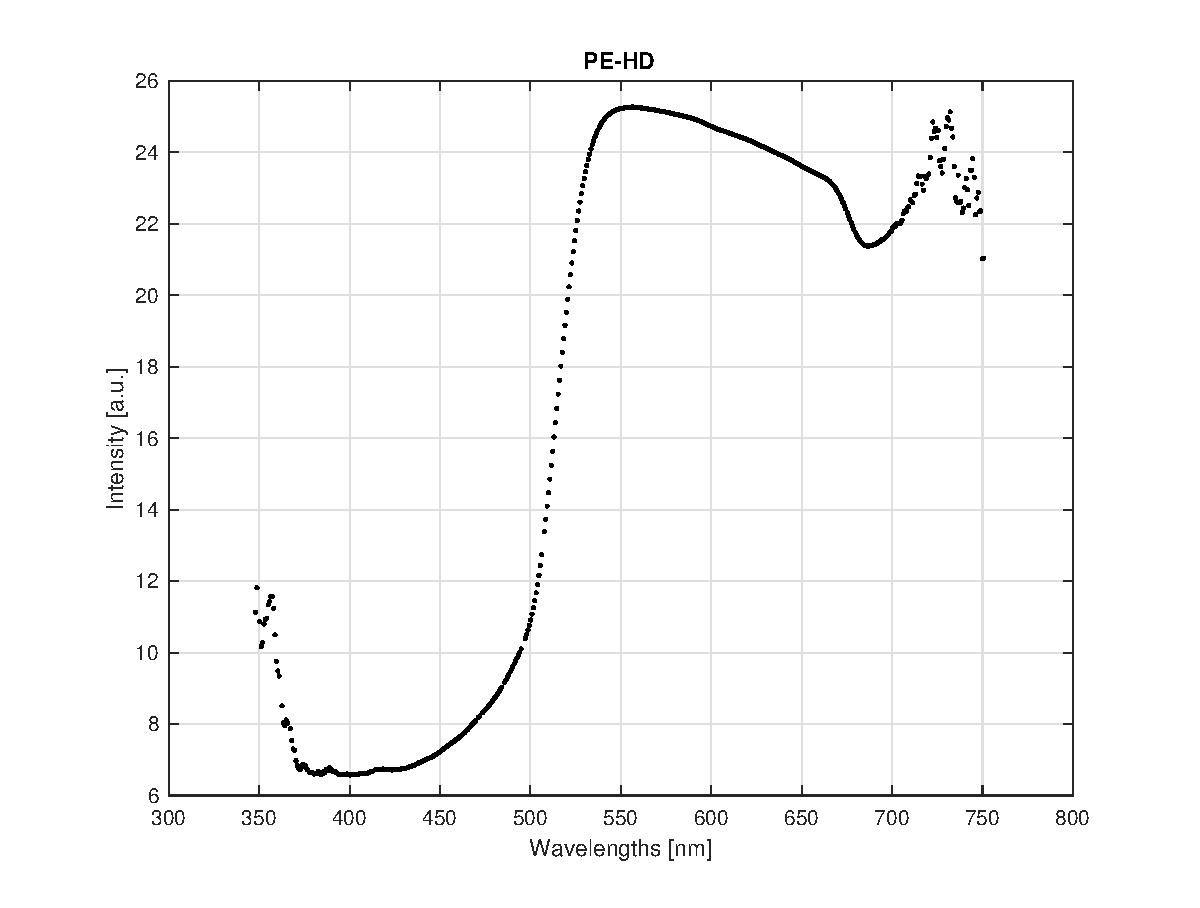
\includegraphics[scale=0.36]{Images/appendix/pe-hd-postconsum.eps}}
  \begin{minipage}{\wd\FigBox}
    \centering\usebox{\FigBox}
    \subcaption{b) PE-HD Post Consumer}
  \end{minipage}
  % Save second image 
  \caption{A comparison of the resulting signature for  and PVC - both in a yellow color}
  \label{fig:plastcomp1}
\end{figure}
\end{comment}


\noindent
As can be seen from Figure \ref{fig:plastcomp1}, the signatures of the two types are almost identical, with a possibility of deviations due to measurements errors. From section \ref{sec:microplastic}, we know for a fact that the structure of these two are very different. PP contains several molecules with the chemical formula of $C_3H_6$, while PVC has molecules with the following formula, $C_2H_3Cl$, even containing additional chlorine-atoms, Cl.  
\\\\
\subsection{Various Colors}
Another result is from the more colorful pieces of microplastics. Figure \ref{fig:green}, \ref{fig:red} and \ref{fig:blue} below display the resulting signatures of green-colored PE-HD, red-colored PE-HD and blue-colored PE-LD, with their associated wavelength circled on the visible light spectrum.  
%grønn
\begin{figure}[H]
  \newcommand*\FigVSkip{0.5em}
  \newcommand*\FigHSkip{0.1em}
  \newsavebox\FigBox
  \centering
% Top image is centered, so no need to get width
 \sbox{\FigBox}{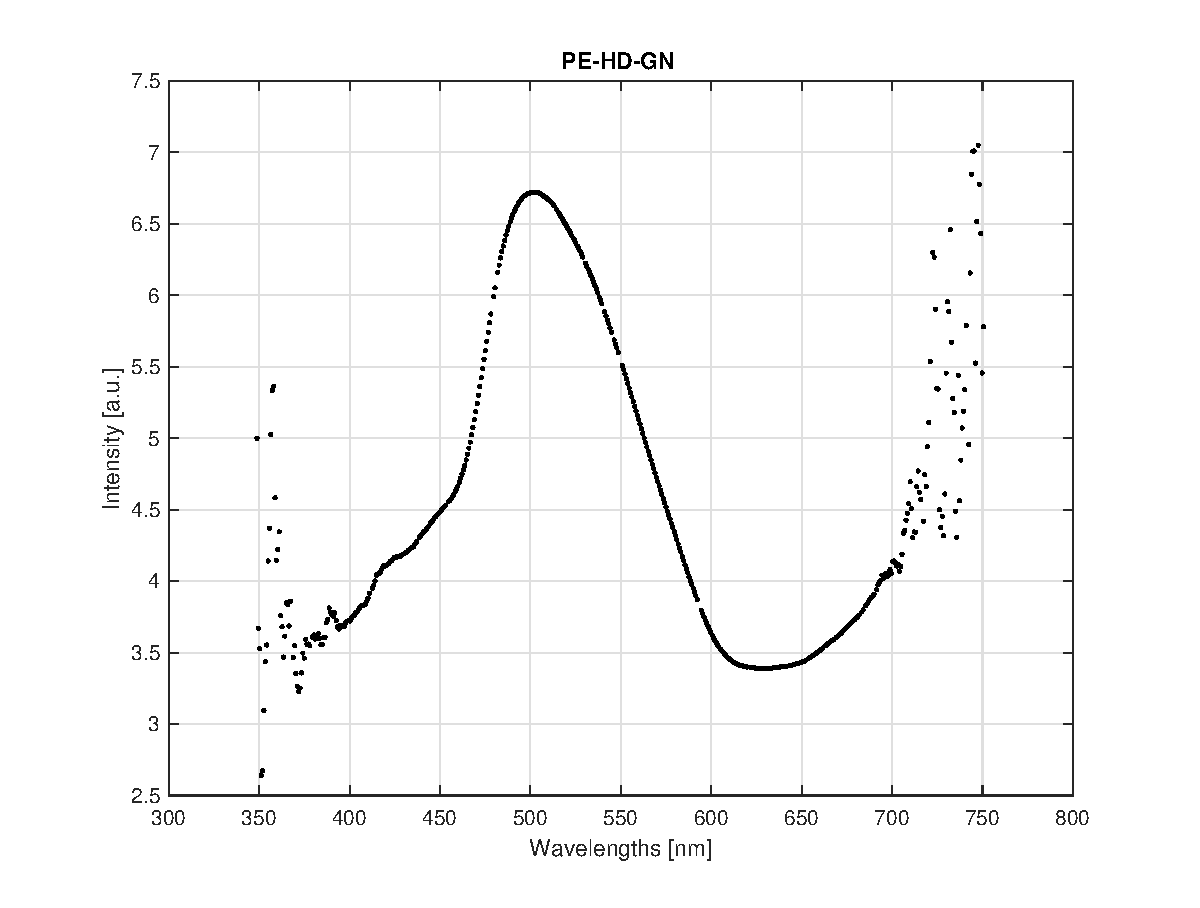
\includegraphics[scale=0.36]{Images/appendix/pe-hd-postconsumer-green.eps}}
  \begin{minipage}{\wd\FigBox}
    \centering\usebox{\FigBox}
    \subcaption{a) PE-HD Post Consumer, Green}
  \end{minipage}
  % Save second image 
  % Top image is centered, so no need to get width
 \sbox{\FigBox}{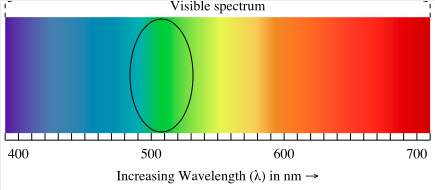
\includegraphics[scale=0.4]{Images/results/specgreen.png}}
  \begin{minipage}{\wd\FigBox}
    \centering\usebox{\FigBox}
    \subcaption{b) The visible light spectrum, circled at green}
  \end{minipage}
  \caption{A comparison of the resulting signature for green-colored PE-HD and the visible light spectrum-reference}
  \label{fig:green}
\end{figure}

%red
\begin{figure}[H]
  \newcommand*\FigVSkip{0.5em}
  \newcommand*\FigHSkip{0.1em}
  \newsavebox\FigBox
  \centering
  % Top image is centered, so no need to get width
 \sbox{\FigBox}{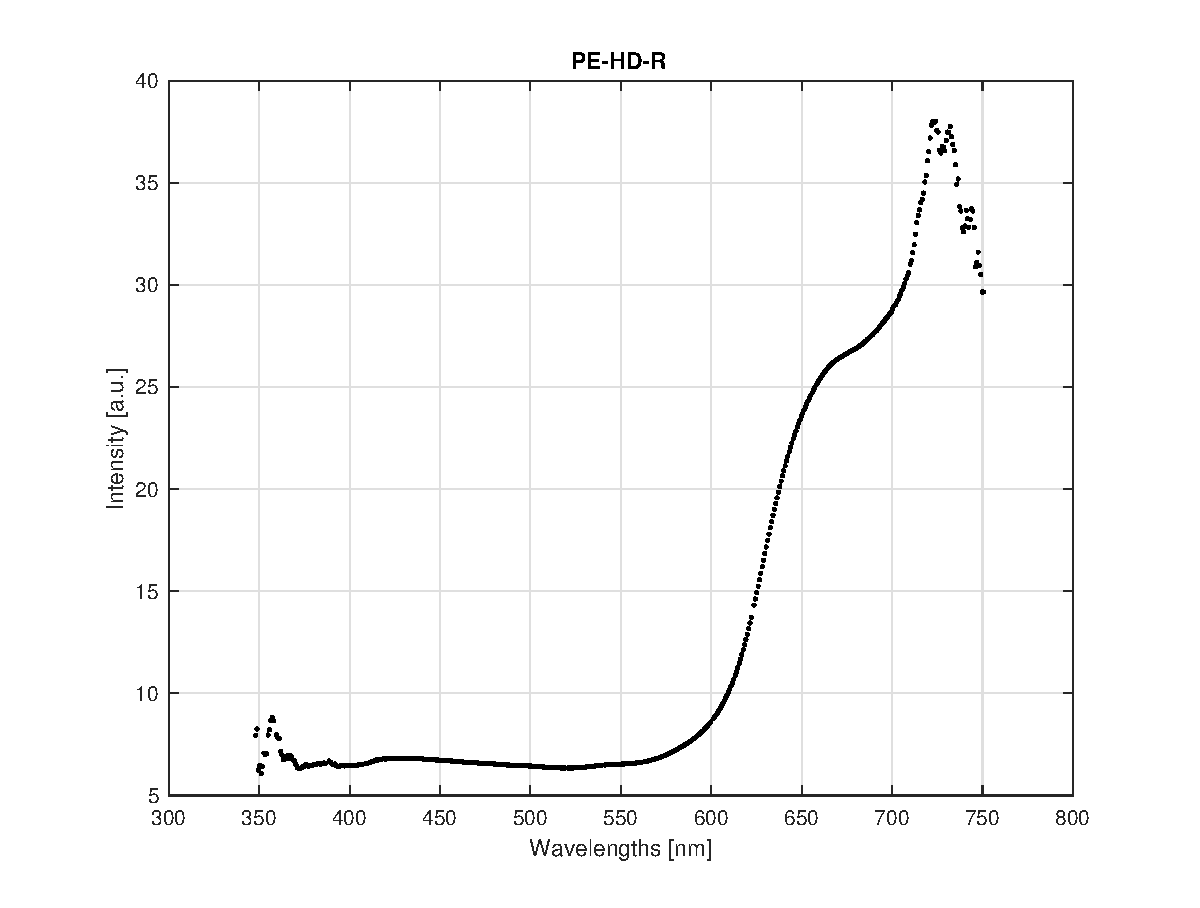
\includegraphics[scale=0.36]{Images/appendix/pe-hd-postconsum-red.eps}}
  \begin{minipage}{\wd\FigBox}
    \centering\usebox{\FigBox}
    \subcaption{a) PE-HD Post Consumer, Red}
  \end{minipage}
    % Top image is centered, so no need to get width
 \sbox{\FigBox}{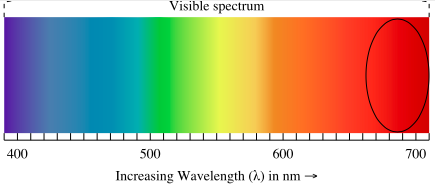
\includegraphics[scale=0.4]{Images/results/specred.png}}
  \begin{minipage}{\wd\FigBox}
    \centering\usebox{\FigBox}
    \subcaption{b) The visible light spectrum, circled at red}
  \end{minipage}
  % Save second image 
  \caption{A comparison of the resulting signature for red-colored PE-HD and the visible light spectrum-reference}
  \label{fig:red}
\end{figure}

%blue
\begin{figure}[H]
  \newcommand*\FigVSkip{0.5em}
  \newcommand*\FigHSkip{0.1em}
  \newsavebox\FigBox
  \centering
  % Top image is centered, so no need to get width
 \sbox{\FigBox}{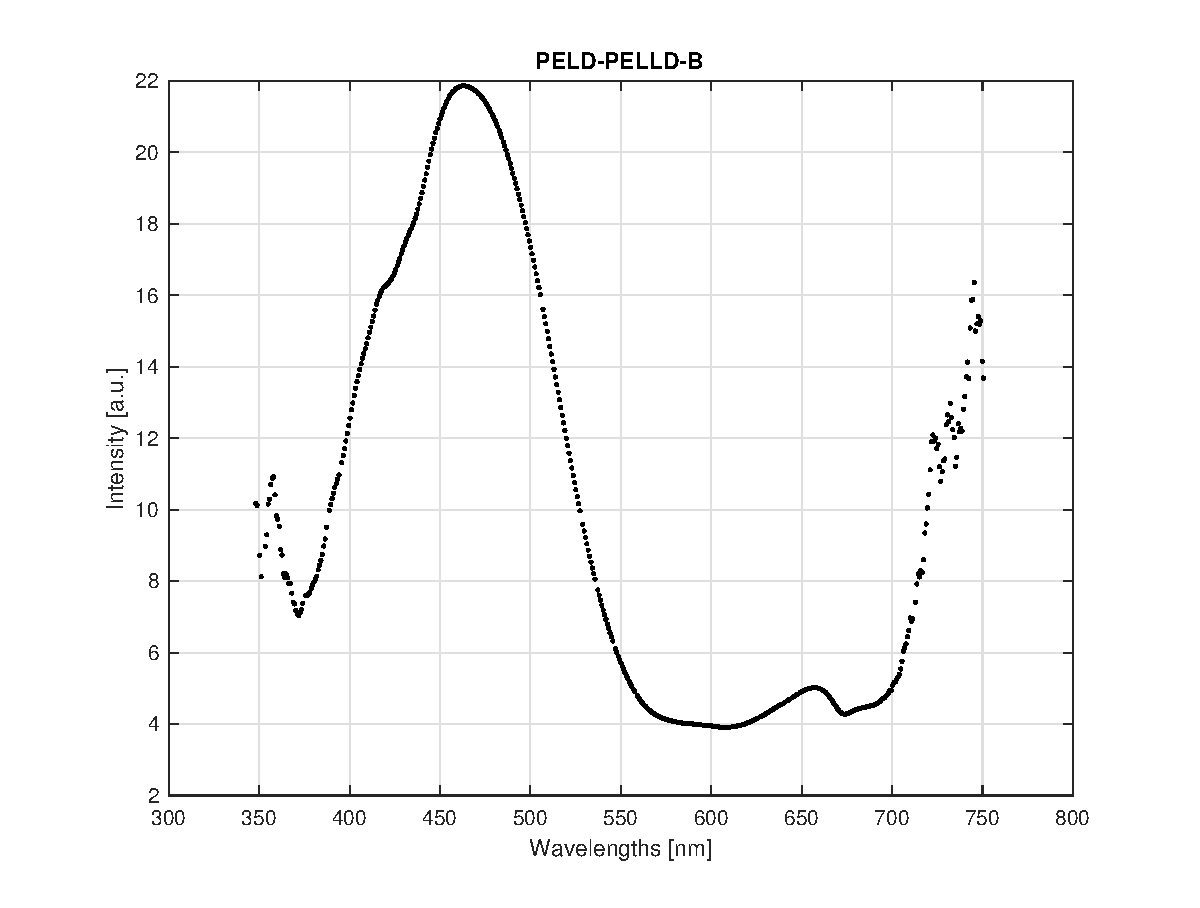
\includegraphics[scale=0.36]{Images/appendix/pe-ld-postindust-blue.eps}}
  \begin{minipage}{\wd\FigBox}
    \centering\usebox{\FigBox}
    \subcaption{a) PE-LD Post Industrial, Blue}
  \end{minipage}
    % Top image is centered, so no need to get width
 \sbox{\FigBox}{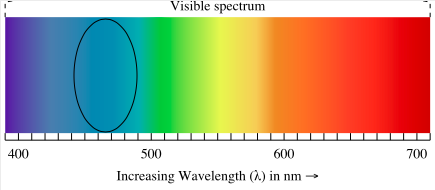
\includegraphics[scale=0.4]{Images/results/specblue.png}}
  \begin{minipage}{\wd\FigBox}
    \centering\usebox{\FigBox}
    \subcaption{b) The visible light spectrum, circled at blue}
  \end{minipage}
  % Save second image 
  \caption{A comparison of the resulting signature for blue-colored PE-LD and the visible light spectrum-reference}
  \label{fig:blue}
\end{figure}

%kilde for visible light reference
%https://www.khanacademy.org/science/physics/light-waves/introduction-to-light-waves/a/light-and-the-electromagnetic-spectrum

\noindent
This result support the earlier assertion about the color being dominant when detecting the spectral image of the plastic. Figure \ref{fig:green} and \ref{fig:red} is even the result of the same type of plastic, PE-HD. However, there is not much resemblance in the plots.
\\\\
The color variation is also found from the PCA as the second principal component. It is therefore reasonable to conclude that the specific color has a large influence.
\\\\
\subsection{Various Sizes}
Another interesting comparison is the result of the same type of plastic, in different sizes. In this section, illustrated by Figure \ref{fig:size}, a clear empty bottle of Farris, existent of PET-plastic, is compared to clear PET Amorphous. The pieces of PET Amorphous are 3mm thick, while the piece from the bottle is significantly larger. 

\begin{figure}[H]
  \newcommand*\FigVSkip{0.5em}
  \newcommand*\FigHSkip{0.1em}
  \newsavebox\FigBox
  \centering
  % Top image is centered, so no need to get width
 \sbox{\FigBox}{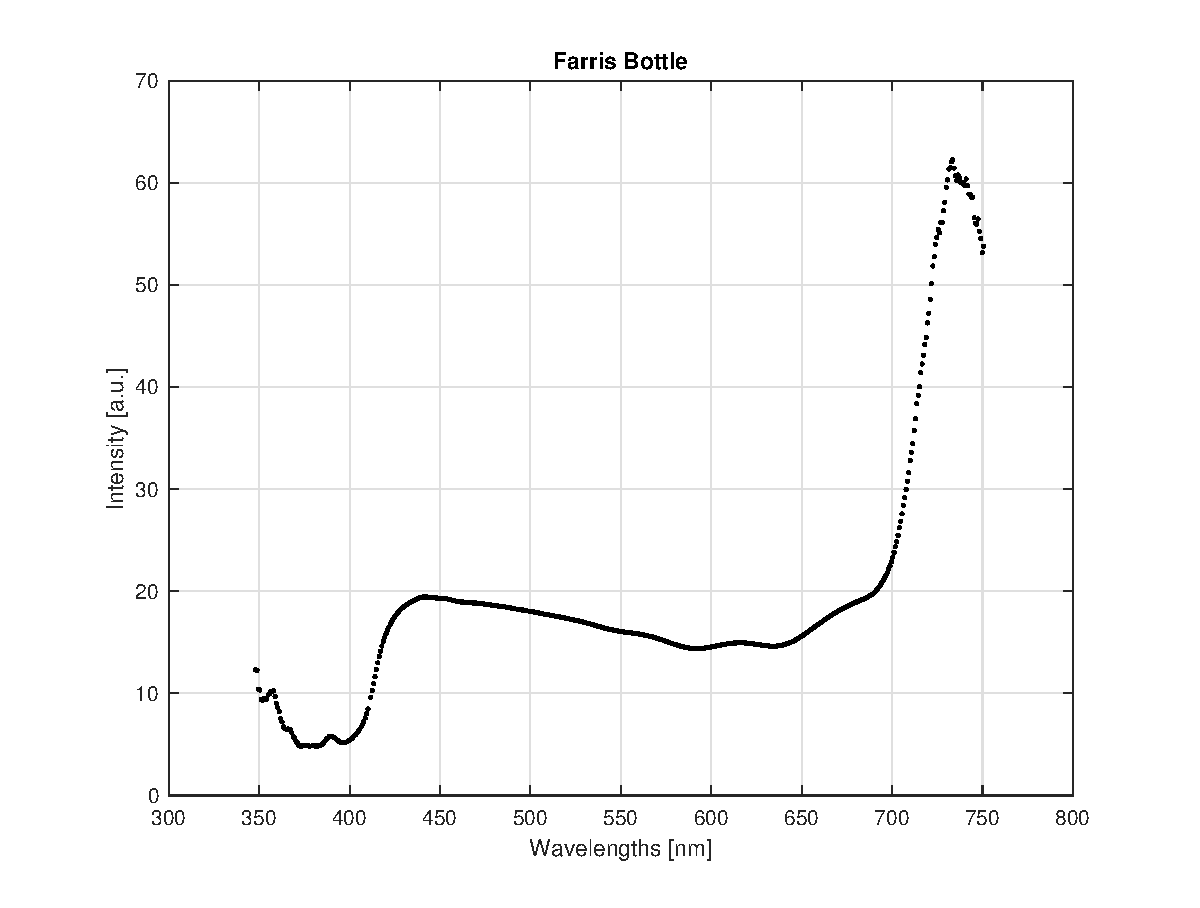
\includegraphics[scale=0.36]{Images/appendix/farris.eps}}
  \begin{minipage}{\wd\FigBox}
    \centering\usebox{\FigBox}
    \subcaption{a) Clear Farris Bottle}
  \end{minipage}
    % Top image is centered, so no need to get width
 \sbox{\FigBox}{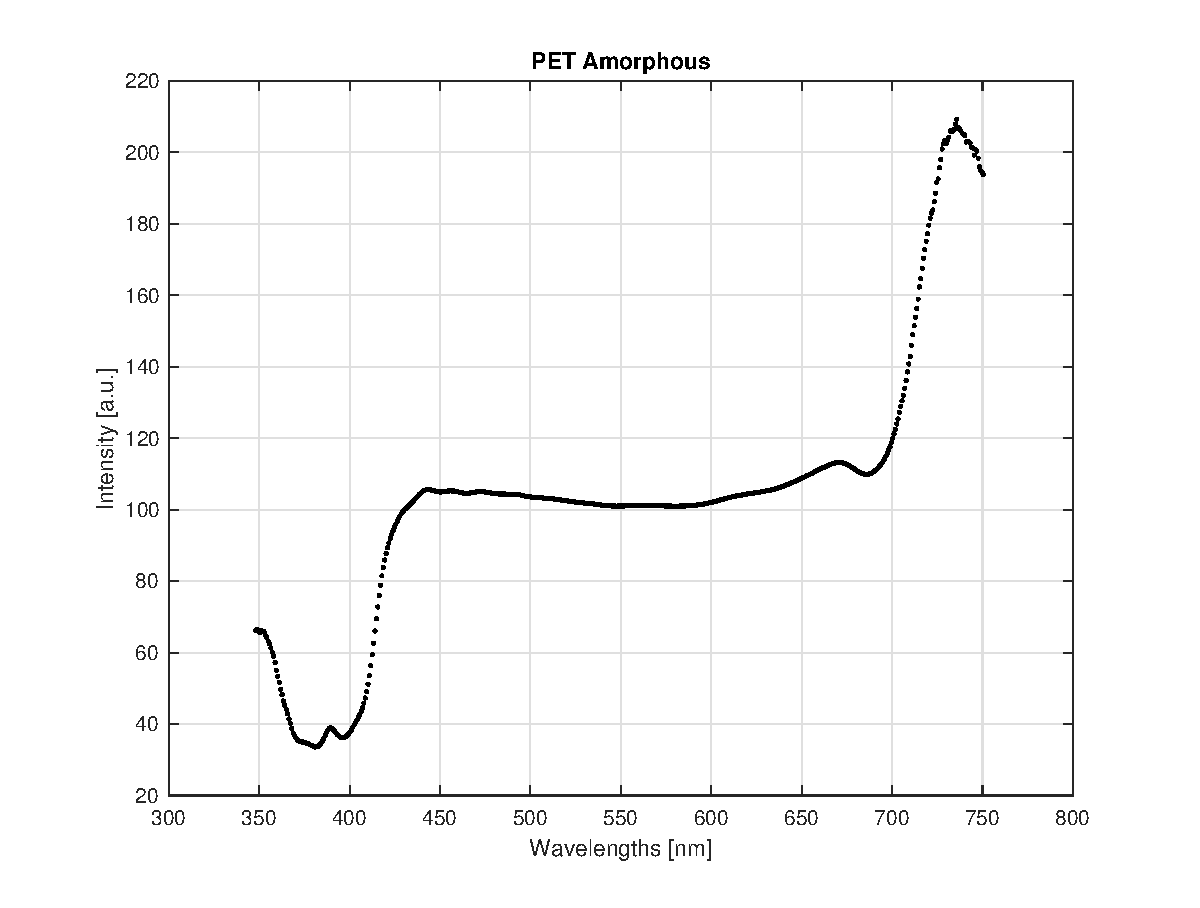
\includegraphics[scale=0.36]{Images/appendix/pet-amorphous-pristine-clear.eps}}
  \begin{minipage}{\wd\FigBox}
    \centering\usebox{\FigBox}
    \subcaption{b) Clear PET Amorphous}
  \end{minipage}
  % Save second image 
  \caption{A comparison of a large PET piece from a Farris bottle and tiny PET Amorphous pieces}
  \label{fig:size}
\end{figure}
\noindent
When comparing the resulting signatures above, it is clear that they share trends. A quick look at the figure reveals many similarities. Nevertheless, looking at the y-axis displaying intensity, one can observe a tripled intensity from the microplastic. 